\documentclass[10pt]{article}
\usepackage{graphicx,booktabs,longtable,array,amsmath,microtype}
\usepackage{jev_journal}
\usepackage[round,authoryear]{natbib}
\usepackage{hyperref}
\hypersetup{colorlinks=true,linkcolor=journalblue,citecolor=journalblue,urlcolor=journalblue}
\renewcommand{\bibsection}{\section*{References}}
\setlength{\bibsep}{4pt}
\title{When Not to Click: Auditing Native Visual Confidence under GUI Target Ambiguity and Distribution Shift}
\author{Anonymous Authors}
\date{}
\begin{document}
\maketitle\thispagestyle{plain}
\begin{abstract}
GUI grounding models can return plausible coordinates when an instruction has no visible or unique target. We audit native presence, match-count and box-confidence signals through synthetic layouts and independently human-labeled real interfaces. A provenance audit removes reused pilot material from the transfer analysis, leaving 751 real-interface cases. On these cases, a three-signal gate accepts 26 actions with 61.5\% conditional error risk; the frozen logistic gate accepts only one action. Strict localization succeeds on 31.3\% of unique targets. A matched-input quantized Qwen baseline provides a separate test of localization and prompted semantic abstention. Label and geometry sensitivity analyses distinguish annotation uncertainty from base-grounder and gate limitations. Real-data recalibration improves probability loss but does not recover a qualifying low-risk operating point under a fixed Learn-then-Test procedure. Native gating succeeds on authored layouts, yet useful automation remains unestablished on this real-interface cohort. We provide traceable source audits, cluster-based uncertainty estimates and reproducible decision analysis; no deployment safety guarantee is claimed.
\end{abstract}
\section*{Introduction}
A screen coordinate answers where a model would click; it does not establish whether the requested control exists or is uniquely identified. Missing, duplicated, occluded and offscreen targets create different decision problems. We study a pinned native visual interface that returns presence, a caller-defined match-count distribution, and one bounding box in a single request.

RQ1: Do native presence and uniqueness scores reduce incorrect accepted clicks relative to box confidence on held-out synthetic layouts? RQ2: How well do the frozen policies transfer to human-labeled real interfaces? RQ3: How do coverage, localization, calibration, latency and cost change across sources and target states? RQ4: How does a frozen local VLM baseline perform on the same images and human references? The contribution is a reproducible audit of a native model interface, its transfer limitations and a matched-input baseline. We do not propose a new uncertainty-control algorithm.

\section*{Related work}
OS-ATLAS develops cross-platform GUI grounding and action modeling \citep{ref1}. SafeGround uses stochastic spatial dispersion and calibration to control false discoveries \citep{ref2}. Argus compares uncertainty methods across models and interfaces, finding that transfer depends on the observable regime \citep{ref3}. CORA learns an action-risk guardian and calibrates execute/abstain behavior \citep{ref4}. Selective classification \citep{ref10}, Learn then Test \citep{ref11} and Conformal Risk Control \citep{ref12} supply the foundational rejection and risk-control framework. Qwen2.5-VL \citep{ref13}, ScreenSpot-Pro \citep{ref14} and UI-TARS \citep{ref15} provide additional GUI-model and benchmark context. These establish prior art for abstention, calibration and GUI safety. Our narrower evidence concerns three native scores from Jev 1.14 and the limitations of a synthetic-to-real evaluation. Published VLM performance is contextualized in Appendix D rather than treated as an experiment on our labels.

\section*{Materials and methods}
\subsection*{Native confidence and selective execution}
Every primary-study request pins jev-1.14.0 with prompt presence-count-box-v1; Appendix C.4 separately specifies the repeat and prompt-variant protocol. Let p be visible-presence confidence, u the Choice probability of exactly one match, and b box confidence. The parser rejects malformed probabilities, unexpected model versions, non-finite coordinates and degenerate boxes. A failed output is an abstention for every policy and remains in evaluation denominators. The selected Choice label is used only to route rejected cases to clarification or abstention; no interactive clarification was executed.

\begingroup\sffamily\fontsize{8}{9.5}\selectfont
\begin{longtable}{>{\raggedright\arraybackslash}p{\dimexpr0.2200\textwidth-2\tabcolsep\relax}>{\raggedright\arraybackslash}p{\dimexpr0.5600\textwidth-2\tabcolsep\relax}>{\raggedright\arraybackslash}p{\dimexpr0.2200\textwidth-2\tabcolsep\relax}}
\caption{Policy definitions. All original thresholds and logistic coefficients remain frozen.}\label{tab:1}\\
\toprule
\textbf{Policy} & \textbf{Score} & \textbf{Threshold}\\\midrule
\endfirsthead
\multicolumn{3}{l}{\small Table \thetable. Continued}\\\toprule
\textbf{Policy} & \textbf{Score} & \textbf{Threshold}\\\midrule
\endhead
A & Every valid parsed box & 0\\
B & b & 0.83\\
C & min(p,b) & 0.83\\
D & min(p,u,b) & 0.80\\
E & sigmoid(-4.496 + 2.509p + 2.696u + 0.600b) & 0.761012\\
Presence & p & 1.00\\
Uniqueness & u & 1.00\\
Presence + uniqueness & min(p,u) & 1.00\\
\bottomrule\end{longtable}\endgroup
E is an L2-regularized logistic regression on the three native scores, fitted to 79 valid development responses. There are no interaction features. Thresholds maximize attainable calibration coverage subject to coverage at most 30\%, breaking ties toward the larger threshold. This is a coverage-selection rule, not a calibrated risk guarantee. No external labels are used to refit these original policies; the "Calibration and decision analysis" subsection reports a separately named real-fitted diagnostic.

\begin{equation}
\tau^*=\arg\max_{\tau}\{\widehat C_{cal}(\tau):\widehat C_{cal}(\tau)\leq0.30\}.
\label{eq:1}
\end{equation}
Let $y_i$=1 only when the target is unique, the predicted center lies in its reference box, and intersection-over-union is at least 0.5. Let $a_i$(t)=1 for a valid output whose score exceeds the threshold; otherwise $a_i$=0. Conditional selective risk and marginal incorrect-action rate have different denominators:

\begin{equation}
\begin{gathered}\widehat C(t)=\frac{1}{n}\sum_i a_i(t)\\[3pt]\widehat R(t)=\frac{\sum_i a_i(t)(1-y_i)}{\sum_i a_i(t)}\\[3pt]\widehat M(t)=\frac{1}{n}\sum_i a_i(t)(1-y_i).\end{gathered}
\label{eq:2}
\end{equation}
Risk is undefined when there are no accepted cases; it is never reported as zero for an empty set. Presence calibration targets the human states unique or multiple; uniqueness calibration targets the unique state. Box and logistic calibration target the full primary correctness criterion. These distinct events must not be interpreted as interchangeable probabilities.

\subsection*{Data, annotation and provenance}
The synthetic pilot has 25 templates in five layout families, eight state variants per template, and procedural geometry labels. Sidebar and kanban form development (80); tables form calibration (40); dialogs and toolbars form held-out test (80). Each template contributes three unique cases and one each of absent, multiple, occluded, offscreen and unclear. The synthetic experiment issued 200 calls without retries; 199 parsed successfully. One development zero-width box failed closed.

Two annotators independently labeled the same 951 cases without model predictions. They chose one of six target states, boxed all valid visible targets for unique/multiple cases, and recorded confidence. Both corrected exports pass structural validation. Status agreement is 759/951 (79.8\%), Cohen's kappa is 0.613, and mean matched box IoU is 0.619 across 205 comparable cases. A deterministic rule flags status disagreement, box-count disagreement, matched IoU below 0.5, or low confidence. It flags 259 cases; reasons overlap. At the authors' direction, the reviewer-approved Annotator B decision is final on flagged cases; the other 692 use consensus and matched-coordinate means where localizable.

An offline source audit finds that 200 of the 951 human-labeled cases reuse exactly the same screenshot bytes and instructions as the pilot: 80 development, 40 calibration and 80 held-out cases. They cannot supply independent external evidence. We therefore report all 951 only as a mixed descriptive cohort, and separately analyze the 751 ScreenSpot-v2-variant real-interface cases \citep{ref8}. The subset analysis was added after inspecting the mixed results, so it is explicitly a post-hoc provenance correction, not a new preregistered experiment. The real subset consists of source-proposed negative instructions rechecked by humans; 131 are ultimately unique, demonstrating why automatic negative labels were insufficient. It is not the standard positive-target ScreenSpot-v2 test set.

\begingroup\sffamily\fontsize{8}{9.5}\selectfont
\begin{longtable}{>{\raggedright\arraybackslash}p{\dimexpr0.2200\textwidth-2\tabcolsep\relax}>{\raggedright\arraybackslash}p{\dimexpr0.1300\textwidth-2\tabcolsep\relax}>{\raggedright\arraybackslash}p{\dimexpr0.1300\textwidth-2\tabcolsep\relax}>{\raggedright\arraybackslash}p{\dimexpr0.1300\textwidth-2\tabcolsep\relax}>{\raggedright\arraybackslash}p{\dimexpr0.1300\textwidth-2\tabcolsep\relax}>{\raggedright\arraybackslash}p{\dimexpr0.1300\textwidth-2\tabcolsep\relax}>{\raggedright\arraybackslash}p{\dimexpr0.1300\textwidth-2\tabcolsep\relax}}
\caption{Cohort composition by frozen human target state. No cases are dropped for schema errors.}\label{tab:2}\\
\toprule
\textbf{Cohort} & \textbf{Unique} & \textbf{Absent} & \textbf{Multiple} & \textbf{Occluded} & \textbf{Offscreen} & \textbf{Unclear}\\\midrule
\endfirsthead
\multicolumn{7}{l}{\small Table \thetable. Continued}\\\toprule
\textbf{Cohort} & \textbf{Unique} & \textbf{Absent} & \textbf{Multiple} & \textbf{Occluded} & \textbf{Offscreen} & \textbf{Unclear}\\\midrule
\endhead
Real interfaces (751) & 131 & 583 & 29 & 2 & 5 & 1\\
Reused synthetic (200) & 75 & 57 & 25 & 25 & 0 & 18\\
Mixed total (951) & 206 & 640 & 54 & 27 & 5 & 19\\
\bottomrule\end{longtable}\endgroup
\begin{figure}[htbp]
\centering
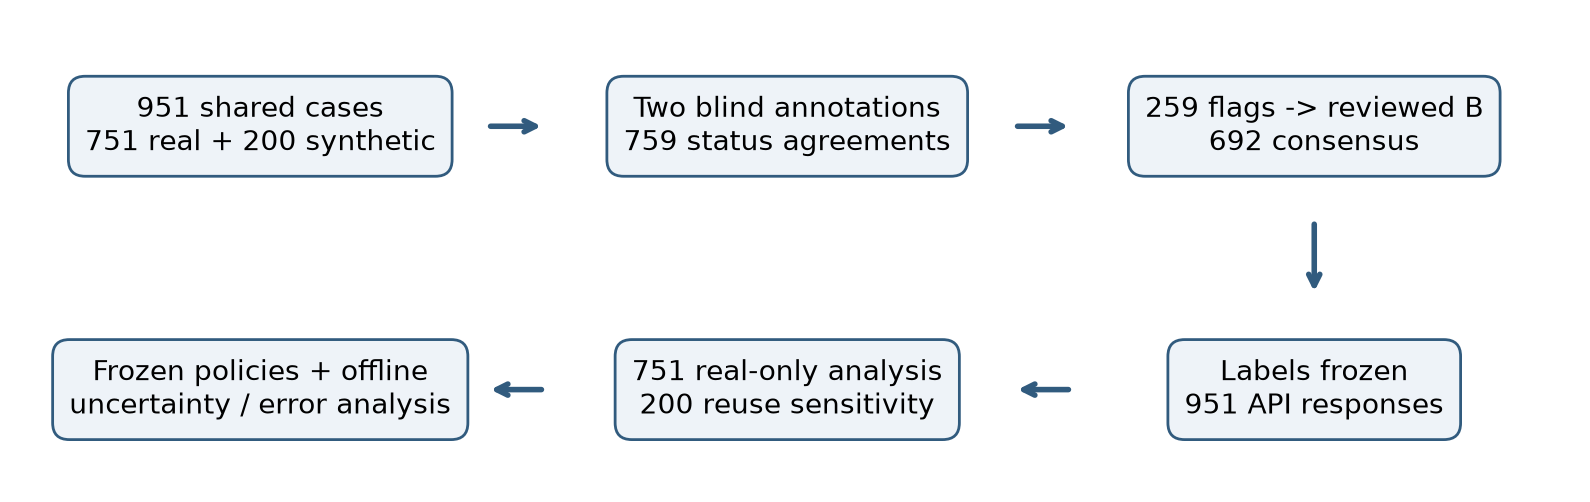
\includegraphics[width=\linewidth,height=3.9in,keepaspectratio]{figures/extended/dataset_flow.png}
\caption{Annotation, source audit and evaluation flow. The real-only analysis separates reused synthetic material.}
\label{fig:1}
\end{figure}
\subsection*{Evaluation and uncertainty protocol}
The main experimental policy definitions remain unchanged. We report strict localization, center-only accuracy as a secondary metric, accepted-error risk, marginal error, state-specific acceptance and useful automation among unique cases. Confidence intervals use 2,000 nonparametric source-image cluster bootstrap resamples with seed 1729. Repeated instructions sharing a screenshot are resampled together. Each ratio is recomputed after resampling, with undefined replicates omitted and their count retained. Primary comparison tests flip paired source-cluster effects and use 10,000 randomizations; Holm adjustment covers the absent and multiple endpoints within each cohort.

The real-only comparisons and all new subgroup, calibration, entropy and curve analyses are exploratory. The absent-target adjusted p=0.0476 is borderline under this exploratory family and carries no central claim. Their two-endpoint Holm adjustment does not cover the full collection of diagnostic analyses. Percentile bootstrap intervals are descriptive and can be unreliable with few accepted cases. A zero-error bootstrap interval is degenerate because resampling cannot create unseen errors; it is not evidence of a true zero risk.

\section*{Results}
\subsection*{Frozen-policy transfer and localization}
\begingroup\sffamily\fontsize{8}{9.5}\selectfont
\begin{longtable}{>{\raggedright\arraybackslash}p{\dimexpr0.2200\textwidth-2\tabcolsep\relax}>{\raggedright\arraybackslash}p{\dimexpr0.1560\textwidth-2\tabcolsep\relax}>{\raggedright\arraybackslash}p{\dimexpr0.1560\textwidth-2\tabcolsep\relax}>{\raggedright\arraybackslash}p{\dimexpr0.1560\textwidth-2\tabcolsep\relax}>{\raggedright\arraybackslash}p{\dimexpr0.1560\textwidth-2\tabcolsep\relax}>{\raggedright\arraybackslash}p{\dimexpr0.1560\textwidth-2\tabcolsep\relax}}
\caption{Primary real-interface results: 751 cases, including 131 unique targets. Original thresholds remain frozen.}\label{tab:3}\\
\toprule
\textbf{Policy} & \textbf{Accept} & \textbf{Errors} & \textbf{Coverage} & \textbf{Risk} & \textbf{Unique automation}\\\midrule
\endfirsthead
\multicolumn{6}{l}{\small Table \thetable. Continued}\\\toprule
\textbf{Policy} & \textbf{Accept} & \textbf{Errors} & \textbf{Coverage} & \textbf{Risk} & \textbf{Unique automation}\\\midrule
\endhead
B & 45 & 28 & 6.0\% & 62.2\% & 13.0\%\\
C & 26 & 17 & 3.5\% & 65.4\% & 6.9\%\\
D & 26 & 16 & 3.5\% & 61.5\% & 7.6\%\\
E & 1 & 0 & 0.1\% & 0.0\% & 0.8\%\\
uniqueness & 2 & 1 & 0.3\% & 50.0\% & 0.8\%\\
\bottomrule\end{longtable}\endgroup
The mixed zero-error logistic result is dominated by reused synthetic inputs: 68 of its 69 accepted cases come from the reused group. On 751 real interfaces, E accepts one correct mobile case (0.13\% coverage). D has 26 accepts and 16 errors (61.5\% risk), versus 45 accepts and 28 errors for B (62.2\% risk). Reducing the absolute number of errors through abstention does not establish lower conditional risk or useful transfer.

For real unique targets, strict localization is correct in 41/131 cases (31.3\%); IoU at least 0.75 occurs in 12/131 (9.2\%), and mean IoU is 0.327. The secondary center-only criterion is satisfied in 77/131 (58.8\%). The large gap illustrates the sensitivity of apparent accuracy to the scoring rule. Box acceptance and safe selection should be evaluated separately.

\begingroup\sffamily\fontsize{8}{9.5}\selectfont
\begin{longtable}{>{\raggedright\arraybackslash}p{\dimexpr0.2200\textwidth-2\tabcolsep\relax}>{\raggedright\arraybackslash}p{\dimexpr0.2600\textwidth-2\tabcolsep\relax}>{\raggedright\arraybackslash}p{\dimexpr0.2600\textwidth-2\tabcolsep\relax}>{\raggedright\arraybackslash}p{\dimexpr0.2600\textwidth-2\tabcolsep\relax}}
\caption{Source-cluster 95\% intervals on the real subset. Risk for E is not inferentially informative.}\label{tab:4}\\
\toprule
\textbf{Policy} & \textbf{Coverage [95\% CI]} & \textbf{Risk [95\% CI]} & \textbf{Useful unique [95\% CI]}\\\midrule
\endfirsthead
\multicolumn{4}{l}{\small Table \thetable. Continued}\\\toprule
\textbf{Policy} & \textbf{Coverage [95\% CI]} & \textbf{Risk [95\% CI]} & \textbf{Useful unique [95\% CI]}\\\midrule
\endhead
B & 6.0\% [4.4\%, 7.7\%] & 62.2\% [47.8\%, 76.0\%] & 13.0\% [7.7\%, 19.1\%]\\
D & 3.5\% [2.2\%, 4.9\%] & 61.5\% [41.7\%, 80.0\%] & 7.6\% [3.6\%, 12.4\%]\\
E & 0.1\% [0.0\%, 0.4\%] & not informative (1 accept) & 0.8\% [0.0\%, 2.4\%]\\
\bottomrule\end{longtable}\endgroup
On real absent targets, B accepts 15/583 and D 7/583, a case-weighted difference of -1.37 points (exploratory two-endpoint Holm-adjusted cluster-sign p=0.0476). On real multiple targets, acceptance changes from 1/29 to 0/29 (adjusted p=1.0). The much larger mixed multiple-target reduction, 21/54 to 0/54, comes mostly from reused synthetic examples. Its mixed-cohort significance does not establish a real-interface ambiguity result.

\begingroup\sffamily\fontsize{8}{9.5}\selectfont
\begin{longtable}{>{\raggedright\arraybackslash}p{\dimexpr0.2200\textwidth-2\tabcolsep\relax}>{\raggedright\arraybackslash}p{\dimexpr0.5600\textwidth-2\tabcolsep\relax}>{\raggedright\arraybackslash}p{\dimexpr0.2200\textwidth-2\tabcolsep\relax}}
\caption{Additional real-subset 95\% source-cluster intervals. A zero-error interval is degenerate, not a guarantee.}\label{tab:5}\\
\toprule
\textbf{Metric} & \textbf{B estimate [95\% CI]} & \textbf{D estimate [95\% CI]}\\\midrule
\endfirsthead
\multicolumn{3}{l}{\small Table \thetable. Continued}\\\toprule
\textbf{Metric} & \textbf{B estimate [95\% CI]} & \textbf{D estimate [95\% CI]}\\\midrule
\endhead
Marginal incorrect-action rate & 3.7\% [2.4\%, 5.1\%] & 2.1\% [1.2\%, 3.3\%]\\
Absent false-accept rate & 2.6\% [1.4\%, 3.9\%] & 1.2\% [0.4\%, 2.2\%]\\
Multiple wrong-accept rate & 3.4\% [0.0\%, 11.1\%] & 0.0\% [0.0\%, 0.0\%]\\
\bottomrule\end{longtable}\endgroup
The completed repeat study reinforces this low-coverage result: across five original-prompt passes, D accepts 21-26 real cases with 57.1-71.4\% conditional risk, while E accepts 0-1 case. Both prewritten prompt variants leave E with no accepts. These repetitions diagnose prediction stability; they do not multiply the number of independent source images. Appendix C.4 reports all pass metrics, failures and additional cost.

\subsection*{Calibration and decision analysis}
Base localization and rejection quality are distinct. Under a center-only rule, real unique-target accuracy rises from 31.3\% to 58.8\%; IoU0.3 alone gives 48.9\%. Among real cases both annotators label unique, only 61.2\% of their boxes meet IoU0.5. These human agreement rates are a conditional reference, not an absolute performance ceiling. Full label/criterion sensitivity appears in Appendix C.1.

An empirical oracle bound makes the base-grounder limitation explicit. For fixed recorded boxes and labels, let $\widehat\pi_{\mathrm{correct}}$ be the fraction of all cases with a strictly correct localization. Any gate has correct-acceptance coverage at most $\widehat\pi_{\mathrm{correct}}$. If its observed conditional error is at most alpha, its total acceptance coverage is at most $\widehat\pi_{\mathrm{correct}}$/(1-alpha). Here $\widehat\pi_{\mathrm{correct}}$=41/751, so even an oracle gate is bounded by about 6.1\% coverage at alpha=0.10. This is a deterministic finite-cohort bound, not a population guarantee or human ceiling; a different grounder or scoring rule changes it.

\begin{equation}
\begin{gathered}\widehat C_{TP}=\frac{1}{n}\sum_i a_i y_i\leq\widehat\pi_{correct}\\[3pt]\widehat R\leq\alpha\Longrightarrow\widehat C\leq\frac{\widehat\pi_{correct}}{1-\alpha}.\end{gathered}
\label{eq:3}
\end{equation}
Original E has Brier loss 0.06125, worse than the retrospective constant-prevalence predictor at 0.05234 (Brier skill -0.170). Its low ECE therefore does not establish useful probability quality. B and E have nearly identical AUROC and overlapping source-cluster intervals; extra native signals do not show strong added discrimination on this real cohort. Appendix C.2 reports the full ranking and Brier analysis.

A source-separated fit/calibration/test diagnostic trains a new logistic score on real fitting data only. Test Brier loss improves from 0.07345 to 0.05822, but neither an empirical calibration-risk rule nor the fixed Learn-then-Test procedure finds a qualifying threshold at 10\% accepted-error risk. This negative recovery result separates improved probability estimation from useful low-risk acceptance. The retrospective design and source-distribution assumptions preclude a new confirmatory guarantee; Appendix C.3 details the procedure.

The appendix reports desktop, mobile and web, status, target-area, element-type, instruction-length, annotator-confidence and label-provenance strata. Target size is reference-box area divided by screenshot area, defined only for unique cases: small below 0.1\%, medium 0.1-1\%, and large at least 1\%. Confidence means the least confident of the two annotators. Sparse strata are descriptive and are not used to tune policies.

\begin{figure}[htbp]
\centering
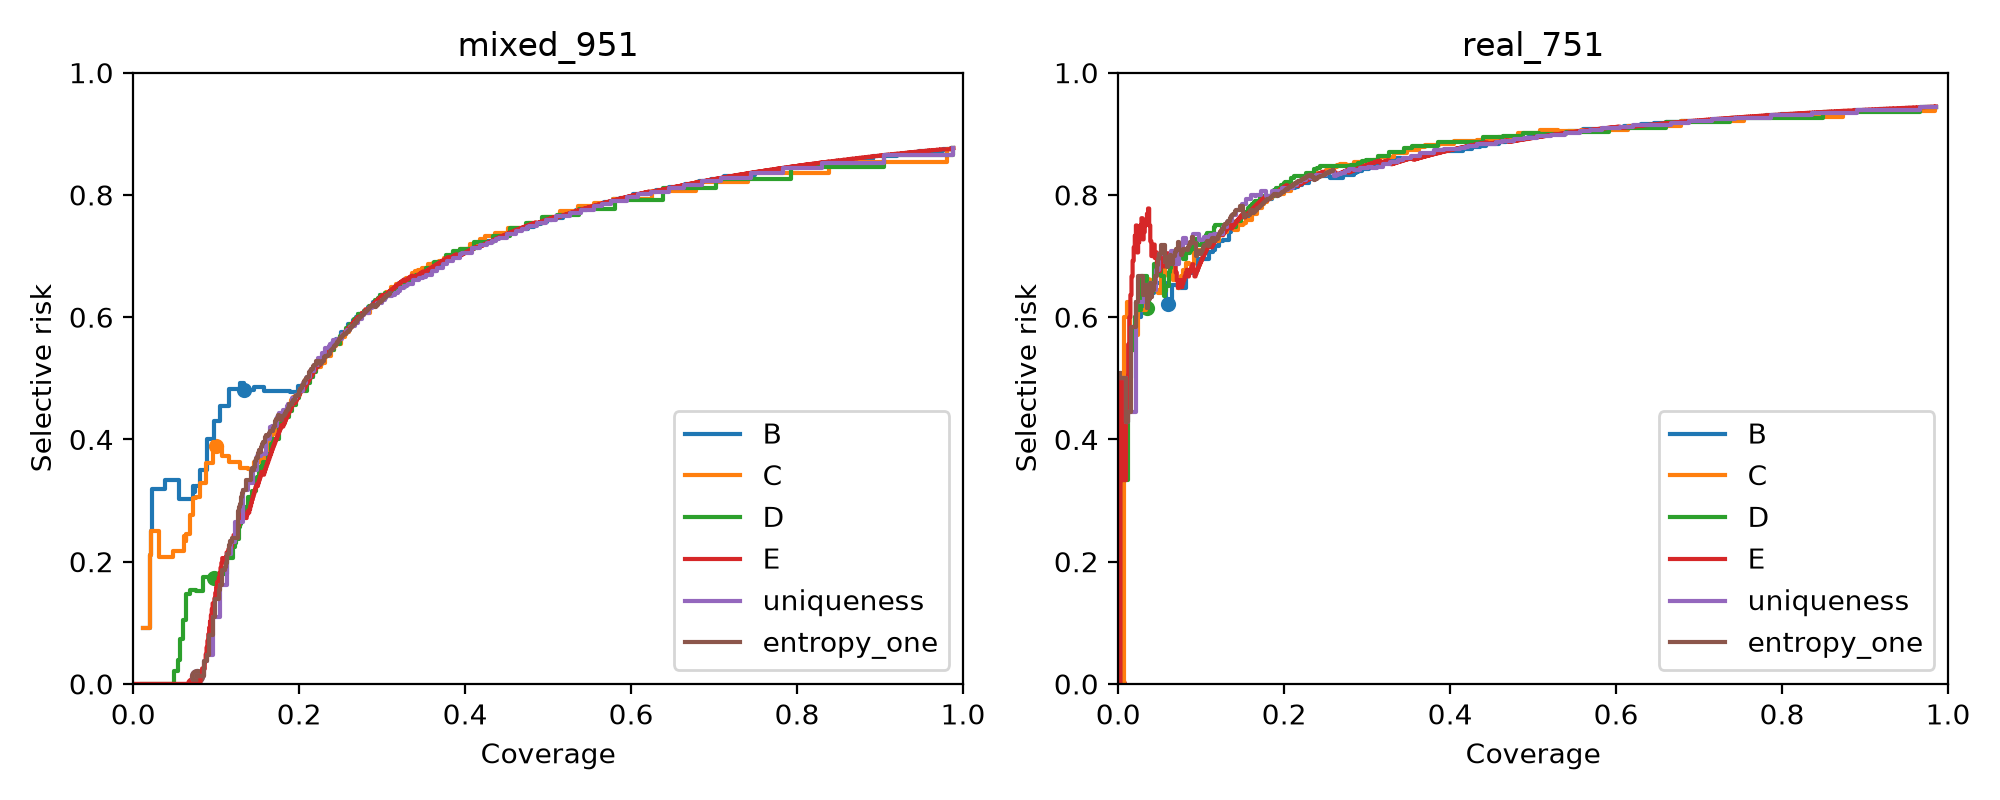
\includegraphics[width=\linewidth,height=3.9in,keepaspectratio]{figures/extended/risk_coverage.png}
\caption{Descriptive risk-coverage sweeps on mixed and real-only cohorts. Dots show the originally frozen operating points. Sweeps inspect test outcomes and cannot be used to select a validated deployment threshold.}
\label{fig:2}
\end{figure}
For an exploratory entropy baseline, h=1-H(q)/log(3), where q is the three-option match-count distribution. A second baseline additionally requires the selected Choice to be one. Their thresholds use only original synthetic calibration outputs at the same 30\% coverage rule, but these baseline designs were introduced after seeing transfer outcomes. Entropy alone selects an infinite threshold and accepts nothing because the tied high-score calibration mass exceeds 30\%. Entropy-plus-one uses threshold 1 and accepts two real cases with one error. Low entropy can mean confidence in absence or multiplicity; it is not equivalent to confidence in a safe click.

\begin{equation}
H(q)=-\sum_{k\in\{0,1,>1\}}q_k\log q_k,\qquad h(q)=1-\frac{H(q)}{\log 3}.
\label{eq:4}
\end{equation}
\begin{figure}[htbp]
\centering
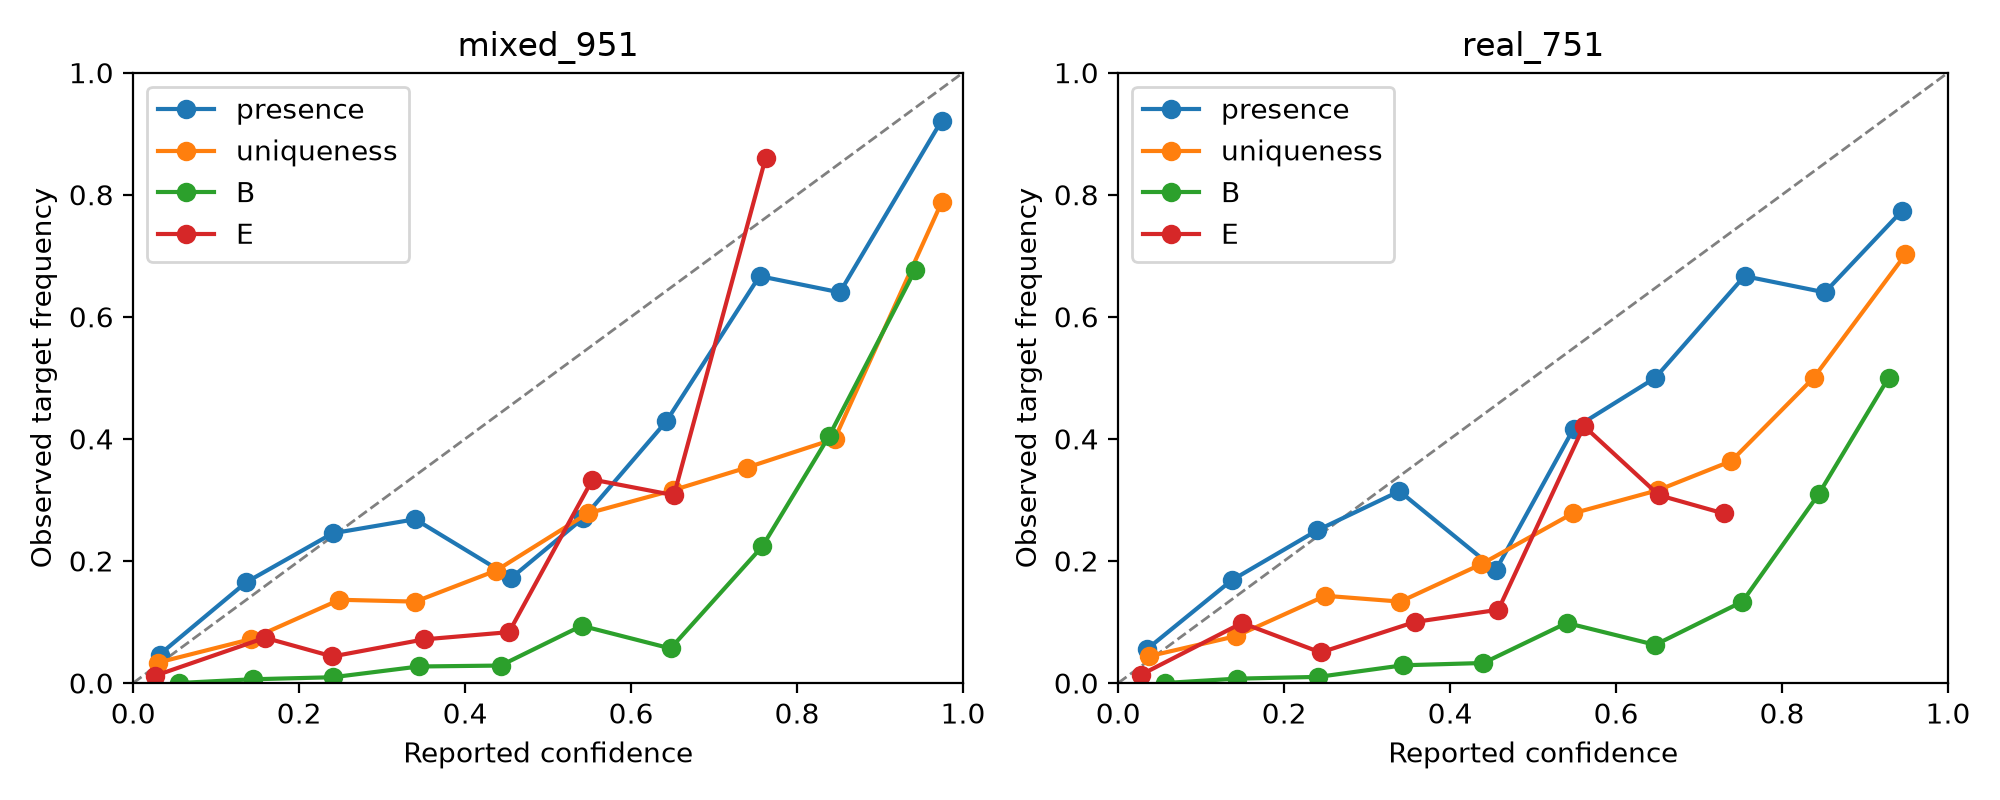
\includegraphics[width=\linewidth,height=3.9in,keepaspectratio]{figures/extended/calibration.png}
\caption{Ten equal-width reliability bins, valid responses only. Different curves target different events, as defined in the "Native confidence and selective execution" subsection; they are not interchangeable calibration comparisons.}
\label{fig:3}
\end{figure}
\begingroup\sffamily\fontsize{8}{9.5}\selectfont
\begin{longtable}{>{\raggedright\arraybackslash}p{\dimexpr0.2200\textwidth-2\tabcolsep\relax}>{\raggedright\arraybackslash}p{\dimexpr0.2600\textwidth-2\tabcolsep\relax}>{\raggedright\arraybackslash}p{\dimexpr0.2600\textwidth-2\tabcolsep\relax}>{\raggedright\arraybackslash}p{\dimexpr0.2600\textwidth-2\tabcolsep\relax}}
\caption{Real-subset calibration on 740 valid responses. Brier and ECE are descriptive, with ten fixed bins.}\label{tab:6}\\
\toprule
\textbf{Score} & \textbf{Event} & \textbf{Brier} & \textbf{ECE}\\\midrule
\endfirsthead
\multicolumn{4}{l}{\small Table \thetable. Continued}\\\toprule
\textbf{Score} & \textbf{Event} & \textbf{Brier} & \textbf{ECE}\\\midrule
\endhead
presence & visible presence & 0.123 & 0.057\\
uniqueness & unique target & 0.143 & 0.130\\
B & correct localization & 0.163 & 0.287\\
E & correct localization & 0.061 & 0.070\\
\bottomrule\end{longtable}\endgroup
As standard decision-theoretic framing rather than a methodological contribution, define a transparent utility: a correct accepted click earns one unit, an incorrect accepted click loses lambda units, and a rejection earns zero. This is a hypothetical sensitivity model, not measured harm. Dollar API cost and wall-clock latency are reported separately.

\begin{equation}
\widehat U_\lambda=\frac{TP-\lambda FP}{n}=\widehat C\,[1-(1+\lambda)\widehat R].
\label{eq:5}
\end{equation}
On real interfaces, $U_B$=(17-28 lambda)/751, $U_D$=(10-16 lambda)/751 and $U_E$=1/751. D exceeds B only when lambda > 7/12; E exceeds D only when lambda > 9/16. A completely abstaining policy has zero utility. These break-even points expose the coverage-risk trade-off rather than labeling one policy universally best.

\begin{equation}
q(x)-\lambda[1-q(x)]\geq0\quad\Longleftrightarrow\quad q(x)\geq\frac{\lambda}{1+\lambda}.
\label{eq:6}
\end{equation}
The last inequality is a Bayes decision derivation under the stated utility. The native scores have not been shown to satisfy its calibration assumptions, so it supplies no guarantee for D or E. Under optimistic independent Bernoulli sampling, zero errors in m accepts yields one-sided 95\% upper bound 1-0.05\textasciicircum{}(1/m). For the single real E acceptance this is 95\%, demonstrating the weakness of that zero-error observation; source dependence makes even this illustration optimistic.

\subsection*{Model comparison, latency and cost}
The independent Qwen2.5-VL-7B baseline uses the same 951 prepared images and human references; input-image hashes and pinned model/protocol hashes match throughout. Primary accuracy uses only the 751 real cases, including 131 unique targets. Qwen uses Q4\_K\_M quantization through Ollama, a frozen forced-box JSON prompt and prompted confidence values; Jev uses its native typed interface. No Jev-trained logistic coefficients are applied to Qwen. These interface and deployment choices delimit the comparison.

\begingroup\sffamily\fontsize{8}{9.5}\selectfont
\begin{longtable}{>{\raggedright\arraybackslash}p{\dimexpr0.2200\textwidth-2\tabcolsep\relax}>{\raggedright\arraybackslash}p{\dimexpr0.1300\textwidth-2\tabcolsep\relax}>{\raggedright\arraybackslash}p{\dimexpr0.1300\textwidth-2\tabcolsep\relax}>{\raggedright\arraybackslash}p{\dimexpr0.1300\textwidth-2\tabcolsep\relax}>{\raggedright\arraybackslash}p{\dimexpr0.1300\textwidth-2\tabcolsep\relax}>{\raggedright\arraybackslash}p{\dimexpr0.1300\textwidth-2\tabcolsep\relax}>{\raggedright\arraybackslash}p{\dimexpr0.1300\textwidth-2\tabcolsep\relax}}
\caption{Observed same-input comparison. Accuracy denominators are 131 unique real targets; timing and failures use all 951 matched inputs. Local total economic cost is unmeasured.}\label{tab:7}\\
\toprule
\textbf{Model / deployment} & \textbf{Strict} & \textbf{Center-only} & \textbf{Failures /951} & \textbf{Mean seconds} & \textbf{p95 seconds} & \textbf{API cost /951}\\\midrule
\endfirsthead
\multicolumn{7}{l}{\small Table \thetable. Continued}\\\toprule
\textbf{Model / deployment} & \textbf{Strict} & \textbf{Center-only} & \textbf{Failures /951} & \textbf{Mean seconds} & \textbf{p95 seconds} & \textbf{API cost /951}\\\midrule
\endhead
Jev HTTP & 31.3\% & 58.8\% & 11 & 0.459 & 0.628 & \$0.1344\\
Qwen Q4 local & 16.8\% & 51.1\% & 62 & 11.339 & 16.667 & \$0 API; compute unpriced\\
\bottomrule\end{longtable}\endgroup
\begin{figure}[htbp]
\centering
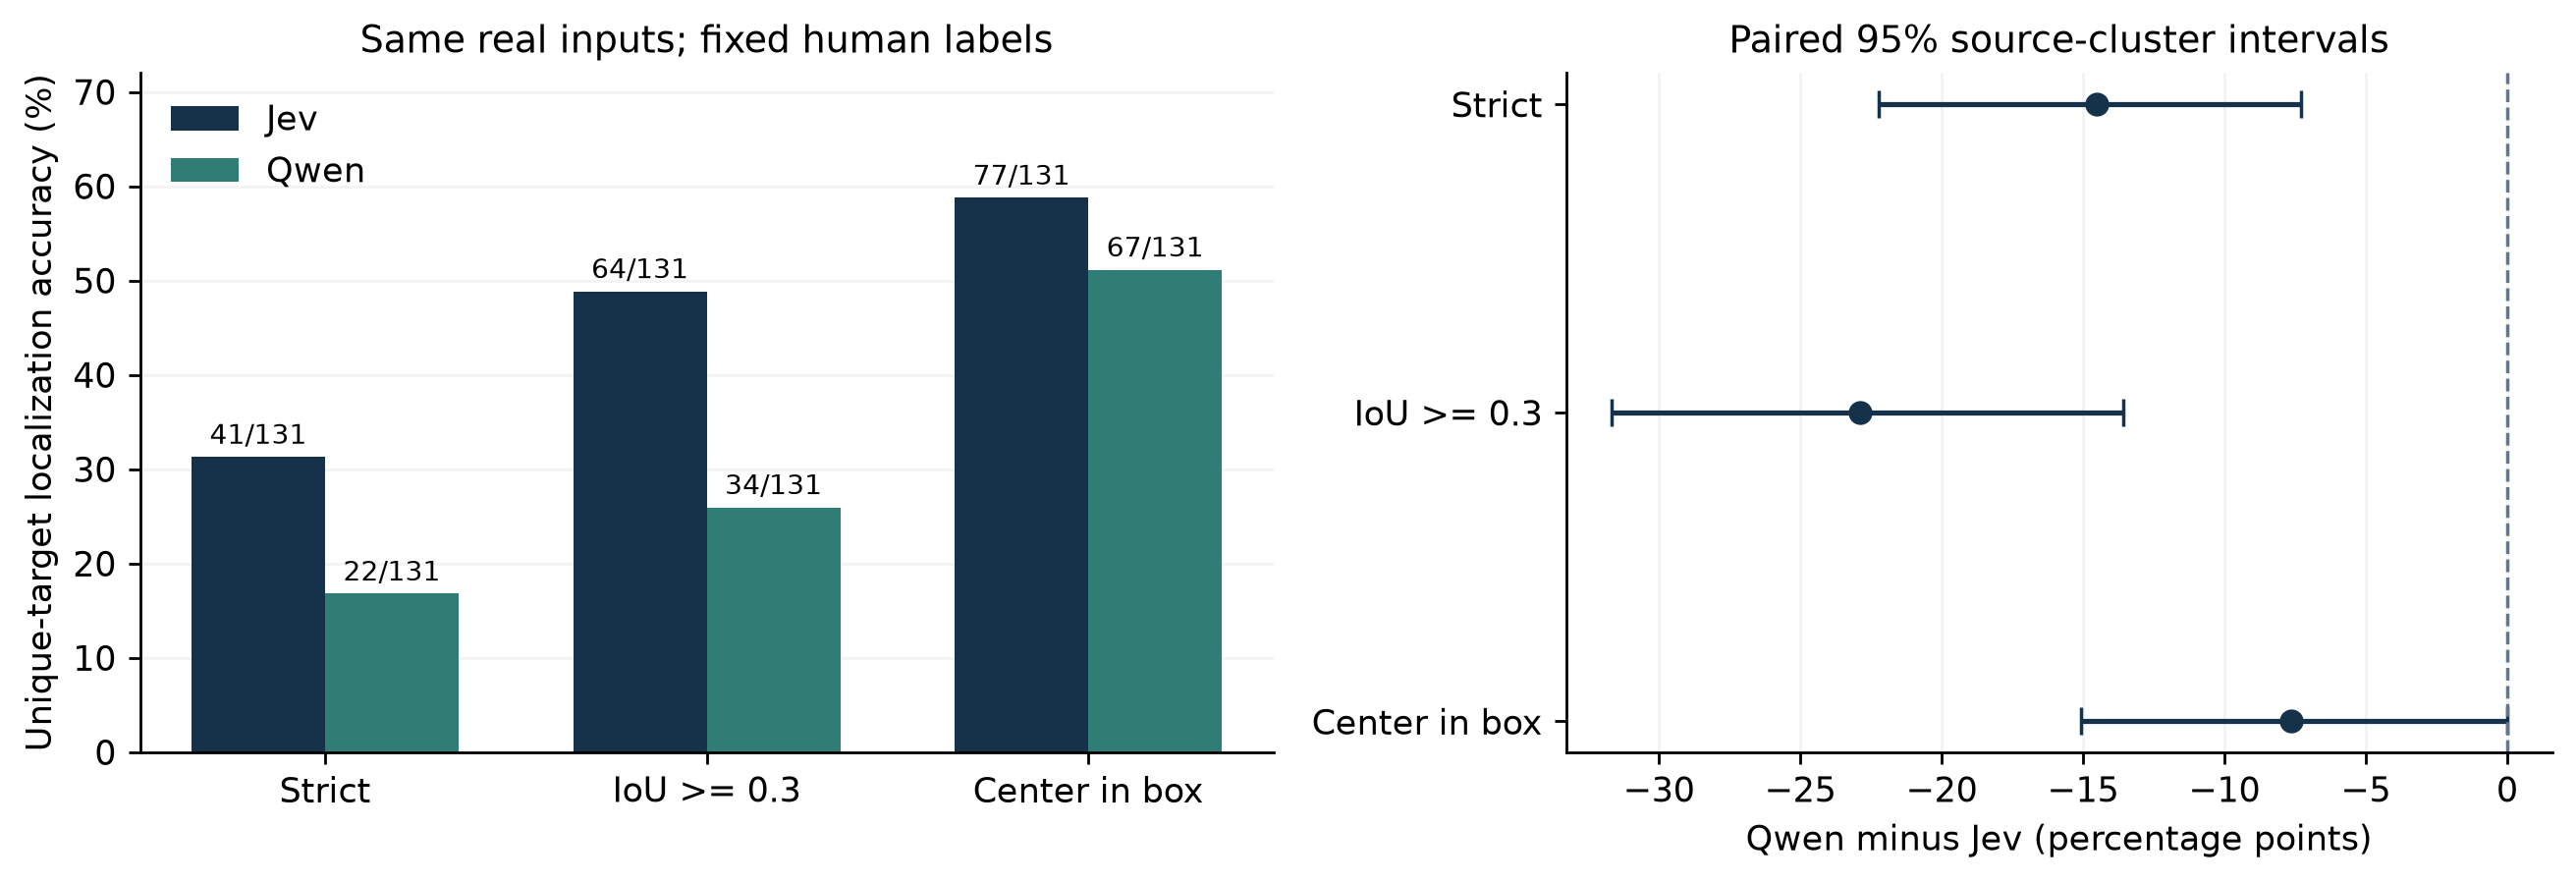
\includegraphics[width=\linewidth,height=3.9in,keepaspectratio]{figures/extended/same_data_comparison.png}
\caption{Observed geometry under the fixed baseline interface. Right: Qwen-minus-Jev differences with 2,000 paired source-image bootstrap resamples. These exploratory intervals are unadjusted across criteria; hardware, quantization and interface effects are not separated.}
\label{fig:4}
\end{figure}
Strict accuracy is 31.3\% for Jev and 16.8\% for Qwen. The paired Qwen-minus-Jev strict difference is -14.5 percentage points (source-cluster 95\% interval -22.2 to -7.3). Center-only accuracy is closer, 58.8\% versus 51.1\%; its difference interval reaches zero. The stricter result favors the tested Jev interface on this cohort, without establishing general model superiority.

A shared semantic rule accepts valid outputs only when the predicted match-count label is one. It accepts 194/751 Jev cases with 163 incorrect accepts, and 604/751 Qwen cases with 583 incorrect accepts. This deliberately simple common rule is separate from frozen policies B-E and shows that a semantic one label alone is insufficient for reliable acceptance. Prompted Qwen scores are not native calibrated probabilities.

The 62 Qwen failures are out-of-bounds or degenerate boxes and remain fail-closed; 57 occur in the real subset. Jev has 11 malformed outputs in the original matched 951 collection, all in the real subset. No output repair or selective rerun was applied. The comparison evaluates the specified forced-box interfaces; it does not isolate model weights, quantization, structured decoding or coordinate-prompt effects. Different model-specific optimization may change results.

Latency is wall-clock request-to-full-response time for each tested deployment. Hosted Jev and serial local Qwen use different hardware and execution stacks; their observed times are not a hardware-normalized speed comparison. Both include malformed-response time. Local Qwen hardware and electricity are unpriced, so zero API charges do not imply zero economic cost. Published model numbers and GPT-4o price scenarios remain historical context in Appendix D.

The external collection contains 951 HTTP-200 responses and 71 earlier credential rejections. Of the former, 940 parse and 11 fail closed: six invalid boxes and five invalid probability sums. Usage must be extracted from raw responses even when parsing fails. Total usage is 3,199,297 input and 73,284 output tokens. Under the recorded Jev input rate of \$0.042 per million tokens, consistent with the provider listing \citep{ref9}, output tokens are listed as free \citep{ref9}. Estimated cost is \$0.134370, or about \$0.0001413 per HTTP-200 response. This is a rate-based estimate rather than a provider invoice. Synthetic-study cost was approximately \$0.019235. Mean valid-or-malformed HTTP-200 latency is 459 ms and p95 628 ms; including setup rejections gives 456 ms mean.

\section*{Discussion}
The central result is the gap between authored-template discrimination and real-interface usefulness. Semantic confidence may successfully reject obvious synthetic duplicates yet fail to transfer to underspecified real instructions and small controls. A low marginal error can be obtained through almost universal abstention. The source audit shows why an apparently strong mixed-cohort result must be decomposed before a generalization claim is made.

Annotations remain a material limitation: status agreement is below 80\%, and final labels for flagged cases follow reviewer-approved B rather than a separate third adjudicator. We cannot infer independent review reliability from this provenance alone. A blinded 100-case audit package (60 flagged and 40 consensus cases) is prepared for a human reviewer. No third-review results are claimed. Changing labels later requires a new dataset version and clearly marked sensitivity analysis.

The real cohort is skewed toward absence (583/751), and unique labels arise from rechecking proposed negative instructions. Mobile, web and desktop are represented, but rare offscreen/occluded strata are too small for stable conclusions. The public training data of Jev are not known, so training contamination cannot be ruled out. Repeated template screenshots are addressed by source-image clustering, but application-level dependence may remain. New subgroup diagnostics were planned after mixed outcomes were visible and have no global multiplicity correction.

The reviewer-driven expansion includes a five-pass Jev study with two prompt variants and a pinned local Qwen2.5-VL collection; completion and results are reported in Appendix C. Both repeatability and same-data baseline collection are complete. The single quantized baseline does not establish robustness across model families or deployment configurations. The present work supplies no formal risk control under distribution shift. Offline incorrect clicks are not measurements of actual user harm, and no real application action was executed. Stronger future evidence requires independent adjudication, new balanced real-interface cases and broader model/configuration coverage.

\section*{Conclusion}
Native uniqueness and presence signals substantially improve selective clicking on authored synthetic layouts, but this result does not establish real-interface usefulness. Removing 200 reused pilot cases reveals that the frozen logistic gate accepts just one of 751 real-interface cases, while three-signal conditional risk remains 61.5\%. The defensible contribution is a transparent account of transfer failure, denominator-sensitive safety metrics and cohort provenance. The matched-input quantized Qwen baseline has weaker observed strict localization under the specified interface, while neither semantic one-label rule yields reliable acceptance. Broader model superiority, formal safety and practical utility remain unestablished.

\section*{Ethics, data availability and reproducibility}
API keys are environment variables and excluded from artifacts. Logs, frozen labels and policies remain unchanged; corrected accounting and post-hoc analyses are versioned separately. External images may contain names or other personal information; screenshots and full annotation exports should remain access-controlled until privacy and source-license review. Public reproducibility material is therefore a manifest/code package with a restricted-data acquisition note, not an unrestricted image redistribution. Author names, affiliations, venue declarations and a public repository URL remain submission-specific tasks.

The artifact contains raw synthetic and external API responses, label exports, source metadata, image-hash overlap audit, per-case decision ledger, full stratified CSVs, 2,000-resample intervals, source-cluster randomization tests, risk-coverage sweeps, reliability bins, cost assumptions, qualitative examples and a shared-content manuscript builder. The offline analysis never imports an API client. A reproduction script runs existing data only, with paid collection commands excluded.

\begin{thebibliography}{99}
\bibitem[Angelopoulos et al.(2024)]{ref12} Angelopoulos, A. N., S. Bates, A. Fisch, L. Lei, and T. Schuster. 2024. Conformal Risk Control. ICLR. \url{https://arxiv.org/abs/2208.02814}
\bibitem[Angelopoulos et al.(2021)]{ref11} Angelopoulos, A. N., S. Bates, E. J. Candes, M. I. Jordan, and L. Lei. 2021. Learn then Test: Calibrating Predictive Algorithms to Achieve Risk Control. arXiv preprint (2021/2022 version history). \url{https://arxiv.org/abs/2110.01052}
\bibitem[Feng et al.(2026)]{ref4} Feng, Y., et al. 2026. CORA: Conformal Risk-Controlled Agents for Safeguarded Mobile GUI Automation. \url{https://arxiv.org/abs/2604.09155}
\bibitem[Geifman and El-Yaniv(2017)]{ref10} Geifman, Y., and R. El-Yaniv. 2017. Selective Classification for Deep Neural Networks. NeurIPS. \url{https://papers.neurips.cc/paper_files/paper/2017/hash/4a8423d5e91fda00bb7e46540e2b0cf1-Abstract.html}
\bibitem[Kumar et al.(2026)]{ref3} Kumar, D., et al. 2026. Uncertainty Quantification for Computer-Use Agents: A Benchmark across Vision-Language Models and GUI Grounding Datasets. \url{https://arxiv.org/abs/2606.25760}
\bibitem[Li, Chen, and Zhang(2026)]{ref5} Li, H., Y. Chen, and Z. Zhang. 2026. GoClick: Lightweight Element Grounding Model for Autonomous GUI Interaction. Table 3 and Section 4.1.2. \url{https://arxiv.org/html/2604.23941v1}
\bibitem[Li et al.(2025)]{ref14} Li, K., et al. 2025. ScreenSpot-Pro: GUI Grounding for Professional High-Resolution Computer Use. \url{https://arxiv.org/abs/2504.07981}
\bibitem[OpenAI(2026a)]{ref6} OpenAI. 2026a. GPT-4o model documentation and pricing. Accessed 23 October 2026. \url{https://developers.openai.com/api/docs/models/gpt-4o}
\bibitem[OpenAI(2026b)]{ref7} OpenAI. 2026b. Images and vision: tile-based image tokenization. Accessed 23 October 2026. \url{https://developers.openai.com/api/docs/guides/images-vision}
\bibitem[Qin et al.(2025)]{ref15} Qin, Y., et al. 2025. UI-TARS: Pioneering Automated GUI Interaction with Native Agents. \url{https://arxiv.org/abs/2501.12326}
\bibitem[Qwen Team(2025)]{ref13} Qwen Team. 2025. Qwen2.5-VL Technical Report. \url{https://arxiv.org/abs/2502.13923}
\bibitem[ScreenSpot-v2-variants(n.d.)]{ref8} ScreenSpot-v2-variants. n.d. Dataset repository. Pinned source revision aa4d83b6833d77d3bb3b7cb769951e2db80052b6. \url{https://huggingface.co/datasets/likaixin/ScreenSpot-v2-variants}
\bibitem[TypeSafe AI(2026)]{ref9} TypeSafe AI. 2026. Introducing System One Models and Jev. Public input/output pricing. Accessed 23 October 2026. \url{https://typesafe.ai/blog/introducing-system-one-models-and-jev}
\bibitem[Wang, Fan, and Wang(2026)]{ref2} Wang, Q., Y. Fan, and X. E. Wang. 2026. SafeGround: Know When to Trust GUI Grounding Models via Uncertainty Calibration. \url{https://arxiv.org/abs/2602.02419}
\bibitem[Wu et al.(2024)]{ref1} Wu, Z., et al. 2024. OS-ATLAS: A Foundation Action Model for Generalist GUI Agents. \url{https://arxiv.org/abs/2410.23218}
\end{thebibliography}
\clearpage
\section*{Appendix A. Additional results and subgroup diagnostics}
\begingroup\sffamily\fontsize{8}{9.5}\selectfont
\begin{longtable}{>{\raggedright\arraybackslash}p{\dimexpr0.2200\textwidth-2\tabcolsep\relax}>{\raggedright\arraybackslash}p{\dimexpr0.1950\textwidth-2\tabcolsep\relax}>{\raggedright\arraybackslash}p{\dimexpr0.1950\textwidth-2\tabcolsep\relax}>{\raggedright\arraybackslash}p{\dimexpr0.1950\textwidth-2\tabcolsep\relax}>{\raggedright\arraybackslash}p{\dimexpr0.1950\textwidth-2\tabcolsep\relax}}
\caption{Held-out synthetic results (80 cases; 30 unique targets).}\label{tab:8}\\
\toprule
\textbf{Policy} & \textbf{Accepted} & \textbf{Incorrect} & \textbf{Risk} & \textbf{Unique automation}\\\midrule
\endfirsthead
\multicolumn{5}{l}{\small Table \thetable. Continued}\\\toprule
\textbf{Policy} & \textbf{Accepted} & \textbf{Incorrect} & \textbf{Risk} & \textbf{Unique automation}\\\midrule
\endhead
B & 27 & 10 & 37.0\% & 56.7\%\\
C & 22 & 5 & 22.7\% & 56.7\%\\
D & 26 & 0 & 0.0\% & 86.7\%\\
E & 29 & 0 & 0.0\% & 96.7\%\\
Uniqueness & 30 & 0 & 0.0\% & 100.0\%\\
\bottomrule\end{longtable}\endgroup
On the synthetic test, B accepts five multiple-target and five occluded cases incorrectly. D and E make no incorrect accepted clicks but reject four and one correctly localized unique cases, respectively. Uniqueness-only accepts all 30 unique targets. The multiple-target B-to-D difference is -50 percentage points; its originally reported Holm-adjusted p=0.126 does not establish significance. The synthetic pilot therefore motivates a transfer check rather than a safety claim.

\begingroup\sffamily\fontsize{8}{9.5}\selectfont
\begin{longtable}{>{\raggedright\arraybackslash}p{\dimexpr0.2200\textwidth-2\tabcolsep\relax}>{\raggedright\arraybackslash}p{\dimexpr0.1560\textwidth-2\tabcolsep\relax}>{\raggedright\arraybackslash}p{\dimexpr0.1560\textwidth-2\tabcolsep\relax}>{\raggedright\arraybackslash}p{\dimexpr0.1560\textwidth-2\tabcolsep\relax}>{\raggedright\arraybackslash}p{\dimexpr0.1560\textwidth-2\tabcolsep\relax}>{\raggedright\arraybackslash}p{\dimexpr0.1560\textwidth-2\tabcolsep\relax}}
\caption{Descriptive mixed-cohort and reused-pilot results. Reuse includes fitting/calibration cases and supplies no independent transfer evidence.}\label{tab:9}\\
\toprule
\textbf{Cohort} & \textbf{Policy} & \textbf{Accept} & \textbf{Errors} & \textbf{Coverage} & \textbf{Risk}\\\midrule
\endfirsthead
\multicolumn{6}{l}{\small Table \thetable. Continued}\\\toprule
\textbf{Cohort} & \textbf{Policy} & \textbf{Accept} & \textbf{Errors} & \textbf{Coverage} & \textbf{Risk}\\\midrule
\endhead
Mixed & B & 127 & 61 & 13.4\% & 48.0\%\\
Mixed & D & 92 & 16 & 9.7\% & 17.4\%\\
Mixed & E & 69 & 0 & 7.3\% & 0.0\%\\
Mixed & uniqueness & 73 & 1 & 7.7\% & 1.4\%\\
Reuse & B & 82 & 33 & 41.0\% & 40.2\%\\
Reuse & D & 66 & 0 & 33.0\% & 0.0\%\\
Reuse & E & 68 & 0 & 34.0\% & 0.0\%\\
Reuse & uniqueness & 71 & 0 & 35.5\% & 0.0\%\\
\bottomrule\end{longtable}\endgroup
\begingroup\sffamily\fontsize{8}{9.5}\selectfont
\begin{longtable}{>{\raggedright\arraybackslash}p{\dimexpr0.2200\textwidth-2\tabcolsep\relax}>{\raggedright\arraybackslash}p{\dimexpr0.1300\textwidth-2\tabcolsep\relax}>{\raggedright\arraybackslash}p{\dimexpr0.1300\textwidth-2\tabcolsep\relax}>{\raggedright\arraybackslash}p{\dimexpr0.1300\textwidth-2\tabcolsep\relax}>{\raggedright\arraybackslash}p{\dimexpr0.1300\textwidth-2\tabcolsep\relax}>{\raggedright\arraybackslash}p{\dimexpr0.1300\textwidth-2\tabcolsep\relax}>{\raggedright\arraybackslash}p{\dimexpr0.1300\textwidth-2\tabcolsep\relax}}
\caption{Platform strata in the mixed cohort; web\_synthetic is explicitly reused. Size applies only to unique cases.}\label{tab:10}\\
\toprule
\textbf{Stratum} & \textbf{Policy} & \textbf{N} & \textbf{Accept} & \textbf{Errors} & \textbf{Coverage} & \textbf{Risk}\\\midrule
\endfirsthead
\multicolumn{7}{l}{\small Table \thetable. Continued}\\\toprule
\textbf{Stratum} & \textbf{Policy} & \textbf{N} & \textbf{Accept} & \textbf{Errors} & \textbf{Coverage} & \textbf{Risk}\\\midrule
\endhead
desktop & B & 235 & 11 & 9 & 4.7\% & 81.8\%\\
desktop & D & 235 & 7 & 6 & 3.0\% & 85.7\%\\
desktop & E & 235 & 0 & 0 & 0.0\% & undefined\\
mobile & B & 258 & 23 & 12 & 8.9\% & 52.2\%\\
mobile & D & 258 & 11 & 5 & 4.3\% & 45.5\%\\
mobile & E & 258 & 1 & 0 & 0.4\% & 0.0\%\\
web & B & 258 & 11 & 7 & 4.3\% & 63.6\%\\
web & D & 258 & 8 & 5 & 3.1\% & 62.5\%\\
web & E & 258 & 0 & 0 & 0.0\% & undefined\\
web\_synthetic & B & 200 & 82 & 33 & 41.0\% & 40.2\%\\
web\_synthetic & D & 200 & 66 & 0 & 33.0\% & 0.0\%\\
web\_synthetic & E & 200 & 68 & 0 & 34.0\% & 0.0\%\\
\bottomrule\end{longtable}\endgroup
\begingroup\sffamily\fontsize{8}{9.5}\selectfont
\begin{longtable}{>{\raggedright\arraybackslash}p{\dimexpr0.2200\textwidth-2\tabcolsep\relax}>{\raggedright\arraybackslash}p{\dimexpr0.1300\textwidth-2\tabcolsep\relax}>{\raggedright\arraybackslash}p{\dimexpr0.1300\textwidth-2\tabcolsep\relax}>{\raggedright\arraybackslash}p{\dimexpr0.1300\textwidth-2\tabcolsep\relax}>{\raggedright\arraybackslash}p{\dimexpr0.1300\textwidth-2\tabcolsep\relax}>{\raggedright\arraybackslash}p{\dimexpr0.1300\textwidth-2\tabcolsep\relax}>{\raggedright\arraybackslash}p{\dimexpr0.1300\textwidth-2\tabcolsep\relax}}
\caption{Target state strata in the mixed cohort; web\_synthetic is explicitly reused. Size applies only to unique cases.}\label{tab:11}\\
\toprule
\textbf{Stratum} & \textbf{Policy} & \textbf{N} & \textbf{Accept} & \textbf{Errors} & \textbf{Coverage} & \textbf{Risk}\\\midrule
\endfirsthead
\multicolumn{7}{l}{\small Table \thetable. Continued}\\\toprule
\textbf{Stratum} & \textbf{Policy} & \textbf{N} & \textbf{Accept} & \textbf{Errors} & \textbf{Coverage} & \textbf{Risk}\\\midrule
\endhead
absent & B & 640 & 15 & 15 & 2.3\% & 100.0\%\\
absent & D & 640 & 7 & 7 & 1.1\% & 100.0\%\\
absent & E & 640 & 0 & 0 & 0.0\% & undefined\\
multiple & B & 54 & 21 & 21 & 38.9\% & 100.0\%\\
multiple & D & 54 & 0 & 0 & 0.0\% & undefined\\
multiple & E & 54 & 0 & 0 & 0.0\% & undefined\\
occluded & B & 27 & 13 & 13 & 48.1\% & 100.0\%\\
occluded & D & 27 & 0 & 0 & 0.0\% & undefined\\
occluded & E & 27 & 0 & 0 & 0.0\% & undefined\\
offscreen & B & 5 & 0 & 0 & 0.0\% & undefined\\
offscreen & D & 5 & 0 & 0 & 0.0\% & undefined\\
offscreen & E & 5 & 0 & 0 & 0.0\% & undefined\\
unclear & B & 19 & 0 & 0 & 0.0\% & undefined\\
unclear & D & 19 & 0 & 0 & 0.0\% & undefined\\
unclear & E & 19 & 0 & 0 & 0.0\% & undefined\\
unique & B & 206 & 78 & 12 & 37.9\% & 15.4\%\\
unique & D & 206 & 85 & 9 & 41.3\% & 10.6\%\\
unique & E & 206 & 69 & 0 & 33.5\% & 0.0\%\\
\bottomrule\end{longtable}\endgroup
\begingroup\sffamily\fontsize{8}{9.5}\selectfont
\begin{longtable}{>{\raggedright\arraybackslash}p{\dimexpr0.2200\textwidth-2\tabcolsep\relax}>{\raggedright\arraybackslash}p{\dimexpr0.1300\textwidth-2\tabcolsep\relax}>{\raggedright\arraybackslash}p{\dimexpr0.1300\textwidth-2\tabcolsep\relax}>{\raggedright\arraybackslash}p{\dimexpr0.1300\textwidth-2\tabcolsep\relax}>{\raggedright\arraybackslash}p{\dimexpr0.1300\textwidth-2\tabcolsep\relax}>{\raggedright\arraybackslash}p{\dimexpr0.1300\textwidth-2\tabcolsep\relax}>{\raggedright\arraybackslash}p{\dimexpr0.1300\textwidth-2\tabcolsep\relax}}
\caption{Target size strata in the mixed cohort; web\_synthetic is explicitly reused. Size applies only to unique cases.}\label{tab:12}\\
\toprule
\textbf{Stratum} & \textbf{Policy} & \textbf{N} & \textbf{Accept} & \textbf{Errors} & \textbf{Coverage} & \textbf{Risk}\\\midrule
\endfirsthead
\multicolumn{7}{l}{\small Table \thetable. Continued}\\\toprule
\textbf{Stratum} & \textbf{Policy} & \textbf{N} & \textbf{Accept} & \textbf{Errors} & \textbf{Coverage} & \textbf{Risk}\\\midrule
\endhead
large (>=1\%) & B & 39 & 9 & 0 & 23.1\% & 0.0\%\\
large (>=1\%) & D & 39 & 7 & 0 & 17.9\% & 0.0\%\\
large (>=1\%) & E & 39 & 2 & 0 & 5.1\% & 0.0\%\\
medium (0.1-1\%) & B & 158 & 66 & 9 & 41.8\% & 13.6\%\\
medium (0.1-1\%) & D & 158 & 75 & 6 & 47.5\% & 8.0\%\\
medium (0.1-1\%) & E & 158 & 67 & 0 & 42.4\% & 0.0\%\\
not\_unique & B & 745 & 49 & 49 & 6.6\% & 100.0\%\\
not\_unique & D & 745 & 7 & 7 & 0.9\% & 100.0\%\\
not\_unique & E & 745 & 0 & 0 & 0.0\% & undefined\\
small (<0.1\%) & B & 9 & 3 & 3 & 33.3\% & 100.0\%\\
small (<0.1\%) & D & 9 & 3 & 3 & 33.3\% & 100.0\%\\
small (<0.1\%) & E & 9 & 0 & 0 & 0.0\% & undefined\\
\bottomrule\end{longtable}\endgroup
\begingroup\sffamily\fontsize{8}{9.5}\selectfont
\begin{longtable}{>{\raggedright\arraybackslash}p{\dimexpr0.2200\textwidth-2\tabcolsep\relax}>{\raggedright\arraybackslash}p{\dimexpr0.1300\textwidth-2\tabcolsep\relax}>{\raggedright\arraybackslash}p{\dimexpr0.1300\textwidth-2\tabcolsep\relax}>{\raggedright\arraybackslash}p{\dimexpr0.1300\textwidth-2\tabcolsep\relax}>{\raggedright\arraybackslash}p{\dimexpr0.1300\textwidth-2\tabcolsep\relax}>{\raggedright\arraybackslash}p{\dimexpr0.1300\textwidth-2\tabcolsep\relax}>{\raggedright\arraybackslash}p{\dimexpr0.1300\textwidth-2\tabcolsep\relax}}
\caption{Annotator confidence strata in the mixed cohort; web\_synthetic is explicitly reused. Size applies only to unique cases.}\label{tab:13}\\
\toprule
\textbf{Stratum} & \textbf{Policy} & \textbf{N} & \textbf{Accept} & \textbf{Errors} & \textbf{Coverage} & \textbf{Risk}\\\midrule
\endfirsthead
\multicolumn{7}{l}{\small Table \thetable. Continued}\\\toprule
\textbf{Stratum} & \textbf{Policy} & \textbf{N} & \textbf{Accept} & \textbf{Errors} & \textbf{Coverage} & \textbf{Risk}\\\midrule
\endhead
high & B & 830 & 117 & 55 & 14.1\% & 47.0\%\\
high & D & 830 & 90 & 15 & 10.8\% & 16.7\%\\
high & E & 830 & 68 & 0 & 8.2\% & 0.0\%\\
low & B & 36 & 4 & 2 & 11.1\% & 50.0\%\\
low & D & 36 & 1 & 0 & 2.8\% & 0.0\%\\
low & E & 36 & 0 & 0 & 0.0\% & undefined\\
medium & B & 85 & 6 & 4 & 7.1\% & 66.7\%\\
medium & D & 85 & 1 & 1 & 1.2\% & 100.0\%\\
medium & E & 85 & 1 & 0 & 1.2\% & 0.0\%\\
\bottomrule\end{longtable}\endgroup
\begingroup\sffamily\fontsize{8}{9.5}\selectfont
\begin{longtable}{>{\raggedright\arraybackslash}p{\dimexpr0.2200\textwidth-2\tabcolsep\relax}>{\raggedright\arraybackslash}p{\dimexpr0.1300\textwidth-2\tabcolsep\relax}>{\raggedright\arraybackslash}p{\dimexpr0.1300\textwidth-2\tabcolsep\relax}>{\raggedright\arraybackslash}p{\dimexpr0.1300\textwidth-2\tabcolsep\relax}>{\raggedright\arraybackslash}p{\dimexpr0.1300\textwidth-2\tabcolsep\relax}>{\raggedright\arraybackslash}p{\dimexpr0.1300\textwidth-2\tabcolsep\relax}>{\raggedright\arraybackslash}p{\dimexpr0.1300\textwidth-2\tabcolsep\relax}}
\caption{Final-label provenance strata in the mixed cohort; web\_synthetic is explicitly reused. Size applies only to unique cases.}\label{tab:14}\\
\toprule
\textbf{Stratum} & \textbf{Policy} & \textbf{N} & \textbf{Accept} & \textbf{Errors} & \textbf{Coverage} & \textbf{Risk}\\\midrule
\endfirsthead
\multicolumn{7}{l}{\small Table \thetable. Continued}\\\toprule
\textbf{Stratum} & \textbf{Policy} & \textbf{N} & \textbf{Accept} & \textbf{Errors} & \textbf{Coverage} & \textbf{Risk}\\\midrule
\endhead
reviewer\_approved\_annotator\_b & B & 259 & 29 & 21 & 11.2\% & 72.4\%\\
reviewer\_approved\_annotator\_b & D & 259 & 18 & 11 & 6.9\% & 61.1\%\\
reviewer\_approved\_annotator\_b & E & 259 & 4 & 0 & 1.5\% & 0.0\%\\
two\_annotator\_consensus & B & 692 & 98 & 40 & 14.2\% & 40.8\%\\
two\_annotator\_consensus & D & 692 & 74 & 5 & 10.7\% & 6.8\%\\
two\_annotator\_consensus & E & 692 & 65 & 0 & 9.4\% & 0.0\%\\
\bottomrule\end{longtable}\endgroup
\begingroup\sffamily\fontsize{8}{9.5}\selectfont
\begin{longtable}{>{\raggedright\arraybackslash}p{\dimexpr0.2200\textwidth-2\tabcolsep\relax}>{\raggedright\arraybackslash}p{\dimexpr0.1300\textwidth-2\tabcolsep\relax}>{\raggedright\arraybackslash}p{\dimexpr0.1300\textwidth-2\tabcolsep\relax}>{\raggedright\arraybackslash}p{\dimexpr0.1300\textwidth-2\tabcolsep\relax}>{\raggedright\arraybackslash}p{\dimexpr0.1300\textwidth-2\tabcolsep\relax}>{\raggedright\arraybackslash}p{\dimexpr0.1300\textwidth-2\tabcolsep\relax}>{\raggedright\arraybackslash}p{\dimexpr0.1300\textwidth-2\tabcolsep\relax}}
\caption{Source element type strata in the mixed cohort; web\_synthetic is explicitly reused. Size applies only to unique cases.}\label{tab:15}\\
\toprule
\textbf{Stratum} & \textbf{Policy} & \textbf{N} & \textbf{Accept} & \textbf{Errors} & \textbf{Coverage} & \textbf{Risk}\\\midrule
\endfirsthead
\multicolumn{7}{l}{\small Table \thetable. Continued}\\\toprule
\textbf{Stratum} & \textbf{Policy} & \textbf{N} & \textbf{Accept} & \textbf{Errors} & \textbf{Coverage} & \textbf{Risk}\\\midrule
\endhead
icon & B & 343 & 19 & 13 & 5.5\% & 68.4\%\\
icon & D & 343 & 8 & 4 & 2.3\% & 50.0\%\\
icon & E & 343 & 1 & 0 & 0.3\% & 0.0\%\\
synthetic\_ui\_element & B & 200 & 82 & 33 & 41.0\% & 40.2\%\\
synthetic\_ui\_element & D & 200 & 66 & 0 & 33.0\% & 0.0\%\\
synthetic\_ui\_element & E & 200 & 68 & 0 & 34.0\% & 0.0\%\\
text & B & 408 & 26 & 15 & 6.4\% & 57.7\%\\
text & D & 408 & 18 & 12 & 4.4\% & 66.7\%\\
text & E & 408 & 0 & 0 & 0.0\% & undefined\\
\bottomrule\end{longtable}\endgroup
\begingroup\sffamily\fontsize{8}{9.5}\selectfont
\begin{longtable}{>{\raggedright\arraybackslash}p{\dimexpr0.2200\textwidth-2\tabcolsep\relax}>{\raggedright\arraybackslash}p{\dimexpr0.1300\textwidth-2\tabcolsep\relax}>{\raggedright\arraybackslash}p{\dimexpr0.1300\textwidth-2\tabcolsep\relax}>{\raggedright\arraybackslash}p{\dimexpr0.1300\textwidth-2\tabcolsep\relax}>{\raggedright\arraybackslash}p{\dimexpr0.1300\textwidth-2\tabcolsep\relax}>{\raggedright\arraybackslash}p{\dimexpr0.1300\textwidth-2\tabcolsep\relax}>{\raggedright\arraybackslash}p{\dimexpr0.1300\textwidth-2\tabcolsep\relax}}
\caption{Instruction length strata in the mixed cohort; web\_synthetic is explicitly reused. Size applies only to unique cases.}\label{tab:16}\\
\toprule
\textbf{Stratum} & \textbf{Policy} & \textbf{N} & \textbf{Accept} & \textbf{Errors} & \textbf{Coverage} & \textbf{Risk}\\\midrule
\endfirsthead
\multicolumn{7}{l}{\small Table \thetable. Continued}\\\toprule
\textbf{Stratum} & \textbf{Policy} & \textbf{N} & \textbf{Accept} & \textbf{Errors} & \textbf{Coverage} & \textbf{Risk}\\\midrule
\endhead
1-3 words & B & 833 & 115 & 52 & 13.8\% & 45.2\%\\
1-3 words & D & 833 & 84 & 10 & 10.1\% & 11.9\%\\
1-3 words & E & 833 & 68 & 0 & 8.2\% & 0.0\%\\
4-7 words & B & 118 & 12 & 9 & 10.2\% & 75.0\%\\
4-7 words & D & 118 & 8 & 6 & 6.8\% & 75.0\%\\
4-7 words & E & 118 & 1 & 0 & 0.8\% & 0.0\%\\
\bottomrule\end{longtable}\endgroup
The machine-readable tables also contain source-dataset strata, all frozen ablations, every state-specific denominator and both mixed/real cohort decompositions. These tables support diagnostic hypotheses rather than independent significance claims. Source element type is metadata about the original target and may not describe the re-labeled counterfactual target.

\section*{Appendix B. Qualitative examples}
Examples are selected deterministically as the first case meeting each stated diagnostic condition, not as a representative sample. Human boxes are green; valid predicted boxes are red. B/D/E indicate frozen accept decisions (1=accept, 0=reject). A box on an absent-target case has no valid human reference box.

\begin{figure}[htbp]
\centering
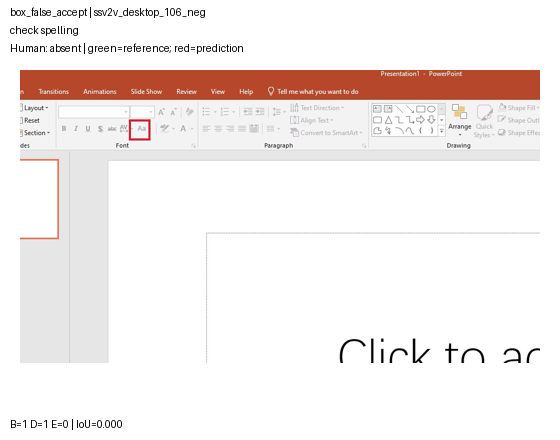
\includegraphics[width=\linewidth,height=3.9in,keepaspectratio]{figures/extended/box_false_accept.png}
\caption{box false accept: ssv2v\_desktop\_106\_neg. Instruction: check spelling. Human status: absent.}
\label{fig:5}
\end{figure}
\begin{figure}[htbp]
\centering
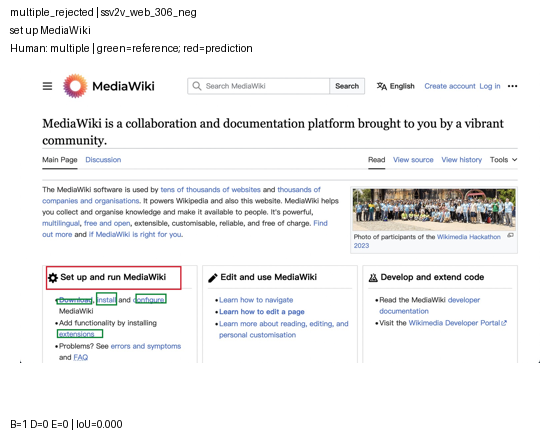
\includegraphics[width=\linewidth,height=3.9in,keepaspectratio]{figures/extended/multiple_rejected.png}
\caption{multiple rejected: ssv2v\_web\_306\_neg. Instruction: set up MediaWiki. Human status: multiple.}
\label{fig:6}
\end{figure}
\begin{figure}[htbp]
\centering
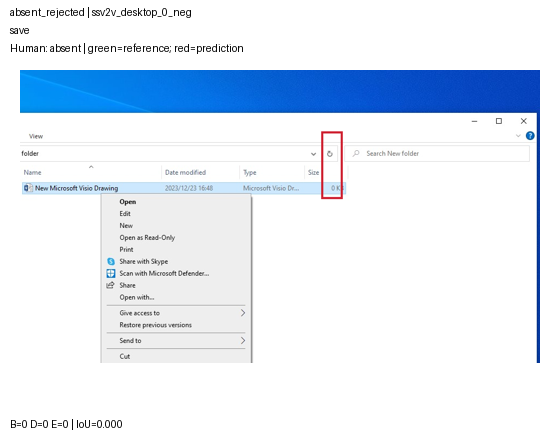
\includegraphics[width=\linewidth,height=3.9in,keepaspectratio]{figures/extended/absent_rejected.png}
\caption{absent rejected: ssv2v\_desktop\_0\_neg. Instruction: save. Human status: absent.}
\label{fig:7}
\end{figure}
\begin{figure}[htbp]
\centering
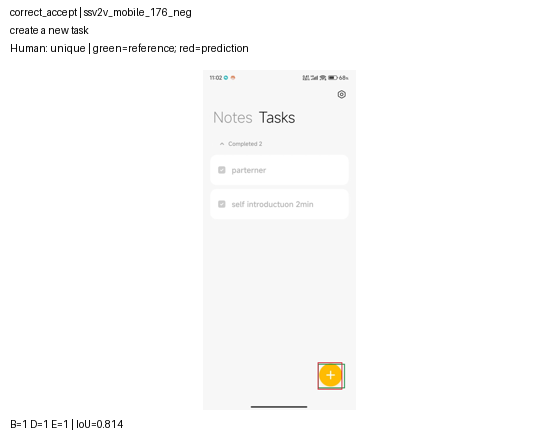
\includegraphics[width=\linewidth,height=3.9in,keepaspectratio]{figures/extended/correct_accept.png}
\caption{correct accept: ssv2v\_mobile\_176\_neg. Instruction: create a new task. Human status: unique.}
\label{fig:8}
\end{figure}
\begin{figure}[htbp]
\centering
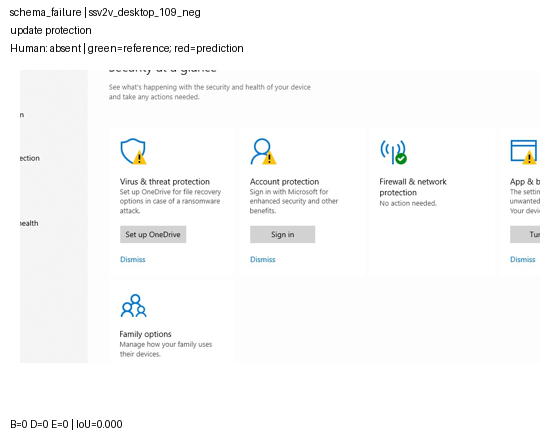
\includegraphics[width=\linewidth,height=3.9in,keepaspectratio]{figures/extended/schema_failure.png}
\caption{schema failure: ssv2v\_desktop\_109\_neg. Instruction: update protection. Human status: absent. Strict parser error: Choice probabilities do not sum to one.}
\label{fig:9}
\end{figure}
\begin{figure}[htbp]
\centering
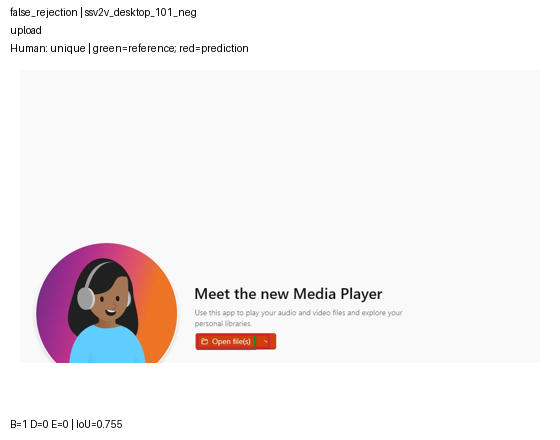
\includegraphics[width=\linewidth,height=3.9in,keepaspectratio]{figures/extended/false_rejection.png}
\caption{false rejection: ssv2v\_desktop\_101\_neg. Instruction: upload. Human status: unique.}
\label{fig:10}
\end{figure}
\section*{Appendix C. Label sensitivity and recalibration}
This expansion was designed after the original real-interface outcomes were inspected. It adds explicit diagnosis of the base grounder, the gate and annotation sensitivity. All original policy definitions and final labels remain frozen. New split-based estimates are exploratory; a retrospective split does not create a previously untouched confirmatory test.

\subsection*{C.1 Label and geometry sensitivity}
\begingroup\sffamily\fontsize{8}{9.5}\selectfont
\begin{longtable}{>{\raggedright\arraybackslash}p{\dimexpr0.2200\textwidth-2\tabcolsep\relax}>{\raggedright\arraybackslash}p{\dimexpr0.1560\textwidth-2\tabcolsep\relax}>{\raggedright\arraybackslash}p{\dimexpr0.1560\textwidth-2\tabcolsep\relax}>{\raggedright\arraybackslash}p{\dimexpr0.1560\textwidth-2\tabcolsep\relax}>{\raggedright\arraybackslash}p{\dimexpr0.1560\textwidth-2\tabcolsep\relax}>{\raggedright\arraybackslash}p{\dimexpr0.1560\textwidth-2\tabcolsep\relax}}
\caption{Frozen accepts evaluated under alternative human references. Consensus-only changes the evaluation population and is not directly comparable in magnitude.}\label{tab:17}\\
\toprule
\textbf{Labels} & \textbf{Policy} & \textbf{N} & \textbf{Accept} & \textbf{Errors} & \textbf{Risk}\\\midrule
\endfirsthead
\multicolumn{6}{l}{\small Table \thetable. Continued}\\\toprule
\textbf{Labels} & \textbf{Policy} & \textbf{N} & \textbf{Accept} & \textbf{Errors} & \textbf{Risk}\\\midrule
\endhead
final & B & 751 & 45 & 28 & 62.2\%\\
final & D & 751 & 26 & 16 & 61.5\%\\
final & E & 751 & 1 & 0 & 0.0\%\\
A\_only & B & 751 & 45 & 22 & 48.9\%\\
A\_only & D & 751 & 26 & 15 & 57.7\%\\
A\_only & E & 751 & 1 & 0 & 0.0\%\\
B\_only & B & 751 & 45 & 28 & 62.2\%\\
B\_only & D & 751 & 26 & 16 & 61.5\%\\
B\_only & E & 751 & 1 & 0 & 0.0\%\\
consensus\_only & B & 515 & 20 & 8 & 40.0\%\\
consensus\_only & D & 515 & 12 & 5 & 41.7\%\\
consensus\_only & E & 515 & 1 & 0 & 0.0\%\\
\bottomrule\end{longtable}\endgroup
A-only and B-only boxes are mapped through the same recorded image scale and padding as the final labels. Consensus-only includes the original two-annotator consensus subset, excluding reviewer-resolved flags. This is an observed sensitivity analysis, not a model-based bound on unknown true risk. The label-dependent error differences show why the pending independent audit matters.

\begingroup\sffamily\fontsize{8}{9.5}\selectfont
\begin{longtable}{>{\raggedright\arraybackslash}p{\dimexpr0.2200\textwidth-2\tabcolsep\relax}>{\raggedright\arraybackslash}p{\dimexpr0.1560\textwidth-2\tabcolsep\relax}>{\raggedright\arraybackslash}p{\dimexpr0.1560\textwidth-2\tabcolsep\relax}>{\raggedright\arraybackslash}p{\dimexpr0.1560\textwidth-2\tabcolsep\relax}>{\raggedright\arraybackslash}p{\dimexpr0.1560\textwidth-2\tabcolsep\relax}>{\raggedright\arraybackslash}p{\dimexpr0.1560\textwidth-2\tabcolsep\relax}}
\caption{Final human labels, real751: localization criterion sensitivity. IoU0.3 uses overlap alone; strict uses center-in-box and IoU0.5.}\label{tab:18}\\
\toprule
\textbf{Criterion} & \textbf{Policy} & \textbf{Correct boxes /131 unique} & \textbf{Accept} & \textbf{Errors} & \textbf{Risk}\\\midrule
\endfirsthead
\multicolumn{6}{l}{\small Table \thetable. Continued}\\\toprule
\textbf{Criterion} & \textbf{Policy} & \textbf{Correct boxes /131 unique} & \textbf{Accept} & \textbf{Errors} & \textbf{Risk}\\\midrule
\endhead
strict & B & 41 & 45 & 28 & 62.2\%\\
strict & D & 41 & 26 & 16 & 61.5\%\\
strict & E & 41 & 1 & 0 & 0.0\%\\
iou03 & B & 64 & 45 & 24 & 53.3\%\\
iou03 & D & 64 & 26 & 12 & 46.2\%\\
iou03 & E & 64 & 1 & 0 & 0.0\%\\
center & B & 77 & 45 & 23 & 51.1\%\\
center & D & 77 & 26 & 11 & 42.3\%\\
center & E & 77 & 1 & 0 & 0.0\%\\
\bottomrule\end{longtable}\endgroup
On 98 real cases that both annotators label unique, mean human-to-human IoU is 0.512. Box agreement reaches IoU0.3 in 79.6\%, IoU0.5 in 61.2\%, and IoU0.75 in 19.4\%. A's box center lies in B's box in 81.6\%; the reverse direction is 88.8\%. These conditional agreement rates are an annotation reference, not an absolute human or model ceiling; they exclude status disagreements and use no independently verified true boxes.

\subsection*{C.2 Brier skill and threshold-free ranking}
\begin{equation}
\mathrm{BSS}=1-\frac{\frac{1}{n}\sum_i(s_i-y_i)^2}{\frac{1}{n}\sum_i(c-y_i)^2}.
\label{eq:7}
\end{equation}
Brier skill is 1 minus the model Brier score divided by a constant-reference Brier score. The retrospective reference predicts the evaluated positive prevalence and is an optimistic in-sample reference. The deployment-oriented reference uses prevalence estimated only from valid real calibration outputs. The all-real $E_{\mathrm{real}}$ row mixes fitting and non-fitting cases and is diagnostic; its test-only row is the relevant recovery estimate.

\begingroup\sffamily\fontsize{8}{9.5}\selectfont
\begin{longtable}{>{\raggedright\arraybackslash}p{\dimexpr0.2200\textwidth-2\tabcolsep\relax}>{\raggedright\arraybackslash}p{\dimexpr0.1560\textwidth-2\tabcolsep\relax}>{\raggedright\arraybackslash}p{\dimexpr0.1560\textwidth-2\tabcolsep\relax}>{\raggedright\arraybackslash}p{\dimexpr0.1560\textwidth-2\tabcolsep\relax}>{\raggedright\arraybackslash}p{\dimexpr0.1560\textwidth-2\tabcolsep\relax}>{\raggedright\arraybackslash}p{\dimexpr0.1560\textwidth-2\tabcolsep\relax}}
\caption{Brier loss and skill under the strict correctness event. Higher skill is better; negative skill is worse than the constant.}\label{tab:19}\\
\toprule
\textbf{Scope} & \textbf{Score} & \textbf{Brier} & \textbf{Retrospective constant} & \textbf{Skill} & \textbf{Calibration-constant skill}\\\midrule
\endfirsthead
\multicolumn{6}{l}{\small Table \thetable. Continued}\\\toprule
\textbf{Scope} & \textbf{Score} & \textbf{Brier} & \textbf{Retrospective constant} & \textbf{Skill} & \textbf{Calibration-constant skill}\\\midrule
\endhead
All valid real & B & 0.1630 & 0.0523 & -2.115 & -2.101\\
All valid real & E & 0.0613 & 0.0523 & -0.170 & -0.165\\
All valid real & $E_{\mathrm{real}}$ & 0.0450 & 0.0523 & 0.141 & 0.145\\
Test valid & B & 0.1591 & 0.0653 & -1.438 & -1.404\\
Test valid & E & 0.0734 & 0.0653 & -0.126 & -0.110\\
Test valid & $E_{\mathrm{real}}$ & 0.0582 & 0.0653 & 0.108 & 0.120\\
\bottomrule\end{longtable}\endgroup
Low ECE alone is insufficient when correct localizations are rare. On all 740 valid real outputs, the constant prevalence is 41/740, whose Brier loss is 0.05234; original E has 0.06125 and skill -0.170. On the exploratory held-out valid subset, real-fitted logistic E improves Brier loss to 0.05822 versus 0.07345 for the original E and 0.06616 for the calibration-prevalence constant, a 12.0\% Brier skill relative to that constant. Probability estimation improves without demonstrating recovery of a 10\%-risk automation policy.

\begingroup\sffamily\fontsize{8}{9.5}\selectfont
\begin{longtable}{>{\raggedright\arraybackslash}p{\dimexpr0.2200\textwidth-2\tabcolsep\relax}>{\raggedright\arraybackslash}p{\dimexpr0.5600\textwidth-2\tabcolsep\relax}>{\raggedright\arraybackslash}p{\dimexpr0.2200\textwidth-2\tabcolsep\relax}}
\caption{Threshold-free metrics on 740 valid real outputs. 1,000 source-cluster resamples give 95\% intervals. AUROC higher and AURC lower are better.}\label{tab:20}\\
\toprule
\textbf{Score} & \textbf{AUROC [95\% CI]} & \textbf{AURC [95\% CI]}\\\midrule
\endfirsthead
\multicolumn{3}{l}{\small Table \thetable. Continued}\\\toprule
\textbf{Score} & \textbf{AUROC [95\% CI]} & \textbf{AURC [95\% CI]}\\\midrule
\endhead
B & 0.869 [0.820, 0.913] & 0.859 [0.816, 0.900]\\
C & 0.843 [0.787, 0.897] & 0.865 [0.825, 0.906]\\
D & 0.837 [0.780, 0.890] & 0.866 [0.825, 0.905]\\
E & 0.869 [0.826, 0.910] & 0.861 [0.820, 0.902]\\
uniqueness & 0.861 [0.810, 0.904] & 0.864 [0.823, 0.904]\\
\bottomrule\end{longtable}\endgroup
AURC integrates right-continuous threshold risk over observed coverage. Equal confidence scores enter together, preventing arbitrary within-tie ordering. Separate machine-readable results include all cases with parser failures placed below valid scores, and the unique-target valid subset. B and E have almost identical AUROC; their overlapping ranking intervals and similar AURC give no evidence that the extra native signals add strong discrimination on this real cohort. AUROC and AURC diagnose ranking, not calibrated risk or downstream harm.

\subsection*{C.3 Real-data recalibration}
\begin{equation}
p_j=\sum_{e=0}^{E_j}\binom{K_j}{e}\alpha^e(1-\alpha)^{K_j-e},\quad p_j\leq\delta/M.
\label{eq:8}
\end{equation}
Source images are assigned deterministically to fit/calibration/test partitions by a seeded hash; no screenshot crosses partitions. The split contains fit: 296 cases/292 source clusters, calibration: 226 cases/218 source clusters, test: 229 cases/220 source clusters. $E_{\mathrm{real}}$ is a new L2 logistic diagnostic fitted on valid fit-partition outputs only; it does not replace the frozen original E.

For Learn then Test \citep{ref11}, the threshold grid is fixed at 0,0.05,...,1. We test the null that conditional accepted-error risk is at least 10\% using a one-sided exact binomial lower-tail p-value. Bonferroni correction covers all 21 thresholds and six scores at overall delta 0.05. To address within-screenshot dependence, one case is independently hash-selected from every source cluster, using no labels. Certified thresholds maximize calibration acceptance within the passing family; if none passes, the procedure abstains. Binomial guarantees target this sampled-cluster distribution and require independent, identically distributed source clusters and a fixed calibration protocol. Those assumptions cannot be fully established retrospectively here, so certification is a diagnostic property of the stated procedure rather than a deployment guarantee.

The empirical comparator maximizes calibration acceptance subject to observed risk at most 10\%, without a statistical guarantee. Neither this comparator nor LTT finds a qualifying threshold for any of the six scores under the strict criterion. Thus the implemented recovery experiment does not show useful automation at the specified 10\% risk target. An alternative risk budget or criterion would require an explicitly separate analysis; it is not selected from test outcomes.

\begingroup\sffamily\fontsize{8}{9.5}\selectfont
\begin{longtable}{>{\raggedright\arraybackslash}p{\dimexpr0.2200\textwidth-2\tabcolsep\relax}>{\raggedright\arraybackslash}p{\dimexpr0.2600\textwidth-2\tabcolsep\relax}>{\raggedright\arraybackslash}p{\dimexpr0.2600\textwidth-2\tabcolsep\relax}>{\raggedright\arraybackslash}p{\dimexpr0.2600\textwidth-2\tabcolsep\relax}}
\caption{Exploratory recovery on 229 test cases. Zero accepts means undefined selective risk, not zero risk.}\label{tab:21}\\
\toprule
\textbf{Score} & \textbf{Empirical accepts} & \textbf{LTT accepts} & \textbf{Incorrect accepts}\\\midrule
\endfirsthead
\multicolumn{4}{l}{\small Table \thetable. Continued}\\\toprule
\textbf{Score} & \textbf{Empirical accepts} & \textbf{LTT accepts} & \textbf{Incorrect accepts}\\\midrule
\endhead
B & 0 & 0 & 0\\
C & 0 & 0 & 0\\
D & 0 & 0 & 0\\
E & 0 & 0 & 0\\
uniqueness & 0 & 0 & 0\\
$E_{\mathrm{real}}$ & 0 & 0 & 0\\
\bottomrule\end{longtable}\endgroup
The source-selected test unit has 220 cases; full 229-case test metrics are also retained descriptively. Recalibration can improve probabilities and alter rejection thresholds, but it cannot create correct boxes that the grounder did not produce. At most 41/131 real unique cases satisfy the strict localization rule in the original pass. This separates weak base localization from a claim that rejection itself is wrong.

\subsection*{C.4 Repeatability and model comparison}
The new Jev protocol fixes four additional original-prompt passes on 751 real cases, yielding five passes including the existing one, plus two prewritten prompt variants. It therefore plans 4,506 additional requests. New requests use separate repeat/prompt IDs and immutable protocol hashes; non-auth attempted IDs, including timeouts and malformed outputs, are not silently resent. At manuscript generation, 7/7 complete pass/variant cohorts are available, including the existing original pass. Partial collections are not used for headline metrics.

Across five complete original-prompt passes, correctness changes in 15/751 cases. Mean per-case modal match-count-label fraction is 0.976. Between-pass policy metrics and per-case consistency are retained separately; repeated observations are not pooled as independent screenshots.

The completed additional collection has 4,506 attempts, 67 fail-closed outputs, 16,457,448 input tokens and 346,928 output tokens. Including recorded usage from malformed responses, the additional rate-based cost estimate is \$0.691213; output tokens are free at the recorded provider rate. No failed attempt was automatically repeated.

Across the five original-prompt passes, B accepts 43-47 cases and D 21-26; D conditional error risk ranges 57.1-71.4\%. E accepts 0-1 case. The literal prompt yields 24 D accepts/15 errors, and the conservative prompt yields 32/23. Prompt changes do not recover useful low-risk coverage under these frozen thresholds. These are descriptive within-case repetitions, not additional independent test screens.

The frozen accept decision changes across original-prompt passes for B: 26/751 cases, D: 17/751 cases, E: 1/751 cases. Mean pairwise box IoU across 7,315 valid within-case output pairs is 0.711; pairs involving malformed outputs are excluded from this geometry diagnostic.

\begingroup\sffamily\fontsize{8}{9.5}\selectfont
\begin{longtable}{>{\raggedright\arraybackslash}p{\dimexpr0.2200\textwidth-2\tabcolsep\relax}>{\raggedright\arraybackslash}p{\dimexpr0.1950\textwidth-2\tabcolsep\relax}>{\raggedright\arraybackslash}p{\dimexpr0.1950\textwidth-2\tabcolsep\relax}>{\raggedright\arraybackslash}p{\dimexpr0.1950\textwidth-2\tabcolsep\relax}>{\raggedright\arraybackslash}p{\dimexpr0.1950\textwidth-2\tabcolsep\relax}}
\caption{Completed Jev pass metrics (751 cases each). Errors are incorrect accepts; malformed responses remain in coverage denominators.}\label{tab:22}\\
\toprule
\textbf{Pass} & \textbf{Policy} & \textbf{Accept} & \textbf{Errors} & \textbf{Risk}\\\midrule
\endfirsthead
\multicolumn{5}{l}{\small Table \thetable. Continued}\\\toprule
\textbf{Pass} & \textbf{Policy} & \textbf{Accept} & \textbf{Errors} & \textbf{Risk}\\\midrule
\endhead
original:r1 & B & 45 & 28 & 62.2\%\\
original:r1 & D & 26 & 16 & 61.5\%\\
original:r1 & E & 1 & 0 & 0.0\%\\
original:r2 & B & 47 & 30 & 63.8\%\\
original:r2 & D & 23 & 14 & 60.9\%\\
original:r2 & E & 1 & 0 & 0.0\%\\
original:r3 & B & 43 & 29 & 67.4\%\\
original:r3 & D & 21 & 13 & 61.9\%\\
original:r3 & E & 1 & 0 & 0.0\%\\
original:r4 & B & 47 & 28 & 59.6\%\\
original:r4 & D & 21 & 12 & 57.1\%\\
original:r4 & E & 1 & 0 & 0.0\%\\
original:r5 & B & 44 & 29 & 65.9\%\\
original:r5 & D & 21 & 15 & 71.4\%\\
original:r5 & E & 0 & 0 & undefined\\
literal:r1 & B & 55 & 39 & 70.9\%\\
literal:r1 & D & 24 & 15 & 62.5\%\\
literal:r1 & E & 0 & 0 & undefined\\
conservative:r1 & B & 37 & 27 & 73.0\%\\
conservative:r1 & D & 32 & 23 & 71.9\%\\
conservative:r1 & E & 0 & 0 & undefined\\
\bottomrule\end{longtable}\endgroup
A same-input local baseline pins Qwen2.5-VL-7B \citep{ref13} through Ollama with model digest recorded, Q4\_K\_M quantization, deterministic decoding, seed 1729, context 4096 and maximum 180 output tokens. The prompt and JSON schema are frozen before the first response. It requests a forced box plus verbalized presence/uniqueness/box-confidence scores. These scores are prompted self-reports rather than native Jev probabilities. Inference is serial on an 18GiB Apple-arm64 Mac. The local compute/energy price is unmeasured, so API charge and total economic cost are not equated.

\begingroup\sffamily\fontsize{8}{9.5}\selectfont
\begin{longtable}{>{\raggedright\arraybackslash}p{\dimexpr0.2200\textwidth-2\tabcolsep\relax}>{\raggedright\arraybackslash}p{\dimexpr0.1560\textwidth-2\tabcolsep\relax}>{\raggedright\arraybackslash}p{\dimexpr0.1560\textwidth-2\tabcolsep\relax}>{\raggedright\arraybackslash}p{\dimexpr0.1560\textwidth-2\tabcolsep\relax}>{\raggedright\arraybackslash}p{\dimexpr0.1560\textwidth-2\tabcolsep\relax}>{\raggedright\arraybackslash}p{\dimexpr0.1560\textwidth-2\tabcolsep\relax}}
\caption{Completed same-data comparison on 751 real cases. Both models use the same prepared images; strict correctness includes eligibility, center and IoU.}\label{tab:23}\\
\toprule
\textbf{Model} & \textbf{Valid} & \textbf{Strict /131 unique} & \textbf{IoU0.3 /131} & \textbf{Center /131} & \textbf{One-label accepts/errors}\\\midrule
\endfirsthead
\multicolumn{6}{l}{\small Table \thetable. Continued}\\\toprule
\textbf{Model} & \textbf{Valid} & \textbf{Strict /131 unique} & \textbf{IoU0.3 /131} & \textbf{Center /131} & \textbf{One-label accepts/errors}\\\midrule
\endhead
Jev & 740 & 41 & 64 & 77 & 194/163\\
Qwen & 694 & 22 & 34 & 67 & 604/583\\
\bottomrule\end{longtable}\endgroup
\begingroup\sffamily\fontsize{8}{9.5}\selectfont
\begin{longtable}{>{\raggedright\arraybackslash}p{\dimexpr0.2200\textwidth-2\tabcolsep\relax}>{\raggedright\arraybackslash}p{\dimexpr0.1950\textwidth-2\tabcolsep\relax}>{\raggedright\arraybackslash}p{\dimexpr0.1950\textwidth-2\tabcolsep\relax}>{\raggedright\arraybackslash}p{\dimexpr0.1950\textwidth-2\tabcolsep\relax}>{\raggedright\arraybackslash}p{\dimexpr0.1950\textwidth-2\tabcolsep\relax}}
\caption{Same-input strict localization under alternative human references. Consensus-only is a smaller selected population, not a noise bound.}\label{tab:24}\\
\toprule
\textbf{Reference} & \textbf{Cases} & \textbf{Unique targets} & \textbf{Jev correct / unique} & \textbf{Qwen correct / unique}\\\midrule
\endfirsthead
\multicolumn{5}{l}{\small Table \thetable. Continued}\\\toprule
\textbf{Reference} & \textbf{Cases} & \textbf{Unique targets} & \textbf{Jev correct / unique} & \textbf{Qwen correct / unique}\\\midrule
\endhead
final & 751 & 131 & 41/131 & 22/131\\
A\_only & 751 & 200 & 55/200 & 18/200\\
B\_only & 751 & 131 & 41/131 & 20/131\\
consensus\_only & 515 & 55 & 20/55 & 15/55\\
\bottomrule\end{longtable}\endgroup
The observed strict-accuracy ordering persists under each reference, while absolute performance and even the number of unique targets vary substantially with annotation choice. This sensitivity is evidence for continued label audit, not proof that any reference is correct. Center-only and IoU0.3 variants are retained in the machine-readable sensitivity table.

Local Qwen request-to-full-response latency is 11.34s mean and 16.67s p95, including the cold first call. This measures the local quantized deployment, not a hosted-Qwen service or a hardware-normalized speed comparison.

All 951 input-image hashes match between Jev and Qwen, and the pinned Qwen model/protocol hashes are unchanged across the resumed collection. The 62 baseline failures all violate box geometry. The completed per-case comparison ledger and paired bootstrap intervals are included in the artifact. Collection was resumed after 446 attempts without repeating earlier logged inputs.

A new source-disjoint candidate pool contains 180 tasks on 60 ScreenSpot-Pro screenshots \citep{ref14}. It has 60 source-positive instructions, 60 cross-application absent candidates and 60 generic multiple-target candidates. File-name and decoded-pixel duplicates against the prior 951 cases are rejected. These are candidate construction categories, not labels; two blind human passes and independent adjudication must establish the final states before confirmatory inference. The professional desktop source is a new domain, not a balanced mobile/web/desktop sample. No model predictions are collected on these candidates before labeling.

The independent 100-case audit (60 flagged, 40 consensus) also remains a human task. Automated analysis and an annotation package cannot substitute for completed human responses. Future labels must create a versioned sensitivity cohort rather than overwrite the frozen experiment.

\section*{Appendix D. Published VLM and price context}
GoClick \citep[Table 3]{ref5} reports standard ScreenSpot-v2 point-grounding results and local timing on one L20 GPU, batch one, 360x780 images. Its task distribution and timing definitions differ from our matched-input experiment. Table values below are historical context rather than new tests or a model ranking.

\begingroup\sffamily\fontsize{8}{9.5}\selectfont
\begin{longtable}{>{\raggedright\arraybackslash}p{\dimexpr0.2200\textwidth-2\tabcolsep\relax}>{\raggedright\arraybackslash}p{\dimexpr0.2600\textwidth-2\tabcolsep\relax}>{\raggedright\arraybackslash}p{\dimexpr0.2600\textwidth-2\tabcolsep\relax}>{\raggedright\arraybackslash}p{\dimexpr0.2600\textwidth-2\tabcolsep\relax}}
\caption{Published model context versus our measurement. Different datasets, metrics and timing definitions prevent a head-to-head ranking.}\label{tab:25}\\
\toprule
\textbf{Model / evidence} & \textbf{Accuracy / scoring set} & \textbf{Timing} & \textbf{Cost evidence}\\\midrule
\endfirsthead
\multicolumn{4}{l}{\small Table \thetable. Continued}\\\toprule
\textbf{Model / evidence} & \textbf{Accuracy / scoring set} & \textbf{Timing} & \textbf{Cost evidence}\\\midrule
\endhead
GPT-4o \citep{ref5} & 20.4\%, standard ScreenSpot-v2 point & Not reported & Official rate \citep{ref6}; scenario below\\
Qwen2VL-7B \citep{ref5} & 66.9\%, same published benchmark & 118.9 ms TTFT; 21.2 ms/token & Local GPU bill not reported\\
UGround \citep{ref5} & 76.5\%, same published benchmark & 1034.6 ms TTFT; 27.9 ms/token & Local GPU bill not reported\\
Jev, our real unique cases & 58.8\% center-only; 31.3\% strict & 459 ms mean full response & Recorded-rate estimate, 951 calls\\
\bottomrule\end{longtable}\endgroup
Published local timings separate time to first token (TTFT) and time per output token (TPOT); our timings measure full HTTP response time. Approximate local generation time is TTFT+(L-1)TPOT for L output tokens, with no comparable GPT-4o timing in the selected study. These values cannot establish a Jev speedup.

For a separate prospective GPT-4o price scenario, official input/output rates \citep{ref6} are \$2.50/\$10 per million tokens. The documented high-detail image rules \citep{ref7} yield 992,205 image tokens for our 951 prepared dimensions. Assuming 250 text-input and 80 output tokens per case gives \$3.835688. These prompt lengths are assumptions, not a measured GPT-4o bill or accuracy result.

\end{document}
